\documentclass[a4paper]{book}
\usepackage{a4wide}
\usepackage{makeidx}
\usepackage{fancyhdr}
\usepackage{graphicx}
\usepackage{multicol}
\usepackage{float}
\usepackage{textcomp}
\usepackage{alltt}
\usepackage{times}
\ifx\pdfoutput\undefined
\usepackage[ps2pdf,
            pagebackref=true,
            colorlinks=true,
            linkcolor=blue
           ]{hyperref}
\usepackage{pspicture}
\else
\usepackage[pdftex,
            pagebackref=true,
            colorlinks=true,
            linkcolor=blue
           ]{hyperref}
\fi
\usepackage{doxygen}
\usepackage{amsmath}
\usepackage{amssymb}
\makeindex
\setcounter{tocdepth}{1}
\renewcommand{\footrulewidth}{0.4pt}
\begin{document}
\begin{titlepage}
\vspace*{7cm}
\begin{center}
{\Large Dr.L. Reference Manual\\[1ex]\large 0.2 }\\
\vspace*{1cm}
{\large Generated by Doxygen 1.3.9.1}\\
\vspace*{0.5cm}
{\small Fri Jun 5 11:11:49 2009}\\
\end{center}
\end{titlepage}
\clearemptydoublepage
\pagenumbering{roman}
\tableofcontents
\clearemptydoublepage
\pagenumbering{arabic}
\chapter{Dimensionality Reduction Library (Dr.L.) }
\label{index}\hypertarget{index}{}\hypertarget{index_intro}{}\section{Introduction}\label{index_intro}
Dr. L. is a C++ library for dimensionality reduction. In the context of this library, dimensionality reduction is considered to consist of: \begin{enumerate}
\end{enumerate}
\begin{enumerate}
\item Estimation of the intrinsic dimensionality using sampled data\item Finding maps that reduce the dimensionality of data (forward map) or increase the dimensionality of data (reverse map). The \char`\"{}find\char`\"{} is performed by optimizing some metric based on the sampled data. In the ideal case, applying the forward map followed by the reverse map should regenerate the original data points.\item Mapping arbitrary coordinates to high and low dimensionalities \end{enumerate}


The library is intended to provide a consistent interface to multiple dimensionality reduction algorithms with an efficient C++ interface that runs efficiently on multicore architectures. A few routines have been optimized with an option for GPU acceleration or distributed computation.

Currently, the library offers intrinsic dimensionality estimation using: \begin{enumerate}
\end{enumerate}
\begin{enumerate}
\item point-PCA\item reconstruction error\item residual variance. \end{enumerate}


The following dimensionality reduction methods have been implemented. \begin{enumerate}
\end{enumerate}
\begin{enumerate}
\item Principal Component Analysis\item Multidimensional Scaling\item Locally Linear Embedding\item Iso\-Map\item Autoencoder Neural Networks \end{enumerate}


An executable is also supplied that can be built to allow for command-line access to the library routines. A description of an application of the library for molecular structure analysis has been published \hyperlink{index_ref}{\mbox{[}Brown, 2009\mbox{]}}.

\par
 \par
 \hypertarget{index_dimred}{}\section{Dimensionality Reduction}\label{index_dimred}
In general, dimensionality reduction algorithms provide a method for taking a set of samples $\{\mathbf{x}_1, \dots, \mathbf{x}_n \} \subset \mathbb{R}^D$ and calculating a corresponding low-dimensional representation $\{\mathbf{y}_1, \dots, \mathbf{y}_n \} \subset \mathbb{R}^d$. Because dimensionality reduction is often used for visualization, some algorithms do not generate an explicit map from the high dimensional coordinates to the low dimensional representation. For many applications, however, it is desirable to have an explicit forward map, $\Phi(\mathbf{x}) : \mathbb{R}^D \rightarrow \mathbb{R}^d$, that gives the low-dimensional representation of an arbitrary point $\mathbf{x}$ and an explicit reverse map $\phi(\mathbf{y}) : \mathbb{R}^d \rightarrow \mathbb{R}^D$ that gives the high-dimensional represenation of an arbitrary point $\mathbf{y}$. This allows for mapping new samples that were not available at the time of the initial reduction and also provides a common metric for comparison of algorithms. Therefore, for the purposes of this work, we consider dimensionality reduction as the problem of generating $\Phi$ and $\phi$ from a training set of $n$ samples, $X_{D \times n} = (\mathbf{x}_1, \dots, \mathbf{x}_n )$. Because some methods do not generate explicit maps, we describe an approach for generating maps from a dimensionality reduction below.

The performance of each algorithm can be evaluated using the reconstruction error. Ideally, a forward map of an arbitrary point followed by a reverse map will give the same point back. Typically, the reconstruction error is given by $\|\mathbf{x}-\phi(\Phi(\mathbf{x}))\|$.

\par
 \par
 \hypertarget{index_ns}{}\section{Namespace}\label{index_ns}
Although hidden from doxygen, the Dr. L. library resides in the {\em yala\/} namespace. You can access Dr. L. commands in your code with the following lines:



\footnotesize\begin{verbatim}#include "dimred/ya_dimred.h"
using namespace yala;
\end{verbatim}
\normalsize


\par
 \par
 \hypertarget{index_vecmat}{}\section{Matrix and Vector Storage in Dr. L.}\label{index_vecmat}
Dr. L. uses a custom linear algebra library for computations. To incorporate the library with your code, wrappers can be used for column-major or row-major matrices stored in traditional continuous memory arrays, STL vectors, or standard library valarrays. The wrapper used will depend on whether each datapoint is stored in a row or a column and whether or not the matrix is column major.



\footnotesize\begin{verbatim}#include "dimred/ya_dimred.h"
using namespace yala;

int main(int argc, char **argv) {
  int rows=4;
  int cols=3;
  int numel=rows*cols;
  double input[numel];
  
  // Fill the matrix....
  
  // If each row is a datapoint (each column is a dimension)
  // --If the matrix is column major
  YA_WRAP(double) input_w(input,rows,cols);
  // --If the matrix is row major
  YA_WRAP_RM(double) input_w(input,rows,cols);
  
  // If each column is a datapoint (each row is a dimension)
  // --If the matrix is column major
  YA_WRAP_RM(double) input_w(input,cols,rows);
  // --If the matrix is row major
  YA_WRAP(double) input_w(input,cols,rows);

  // Use input_w with Dr. L. routines...
  // Same procedure can be used for output matrices.
  
  // Use input as usual...
  
  return 0;
}
\end{verbatim}
\normalsize


For single precision, double is replaced with float in the wrappers above, etc. For STL vectors:



\footnotesize\begin{verbatim}  std::vector<double> input;
  
  ...
  
  
  YA_VWRAP(double) input_w(input.begin(),rows,cols);
  
  // or
  
  YA_VWRAP_RM(double) input_w(input.begin(),rows,cols);
\end{verbatim}
\normalsize


For valarray:



\footnotesize\begin{verbatim}  std::valarray<double> input;
  
  ...
  
  YA_WRAP(double) input_w(&input[0],rows,cols);
  
  // or
  
  YA_WRAP_RM(double) input_w(&input[0],rows,cols);
\end{verbatim}
\normalsize


\par
 \par
 \hypertarget{index_general}{}\section{General Dimensionality Reduction Routines}\label{index_general}
Several general dimensionality reduction routines are available through the pure virtual class \hyperlink{class_y_a_dim_reduce}{YADim\-Reduce}. The base class can also be used for run-time selection of dimensionality routines:



\footnotesize\begin{verbatim}  YADimReduce<double> *redmet=NULL;
  
  if (method_str=="PCA")
    redmet=new YAPCAReduce<double>;
  else if (method_str=="MDS")
    redmet=new YAMDSReduce<double>;
  else if (method_str=="LLE")
    redmet=new YALLEReduce<double>;
  else if (method_str=="ISOMAP")
    redmet=new YAIsoReduce<double>;
  else if (method_str=="AE")
    redmet=new YAATEReduce<double>;
\end{verbatim}
\normalsize


The following sample code describes some of the routines available through the base class:



\footnotesize\begin{verbatim}  // Store the high dimensionality and low dimensionality for maps somewhere
  int high_dim=5;
  int low_dim=3;
  
  // For methods that utilize eigen decomposition, options are set through
  // the EigenOptions class.
  EigenOptions eigopts;
  
  // Set the degree of output to the console
  // -- 0 is not output, 1 outputs a progress meter, 2 also outputs nbor stats
  redmet->verbose(2);

  // The find routine uses a set of input samples to obtain forward and reverse
  // maps. Additionally, this routine will store the low-dimensional 
  // representation for a set of samples in an output matrix. 
  redmet->find_t(input, output, low_dim, eigopts);
  
  // Map in the forward direction to reduce the dimensionality of a matrix
  redmet->forward_t(input_mat, output_mat);
  
  // Map in the reverse direction to increase the dimensionality of a matrix
  redmet->reverse_t(input_mat, output_mat);
  
  // Calculate RMSD representing the reconstruction error from the input matrix
  double err = redmet->reconstruct_error(input);  
    
  // Save dimensionality reduction maps to the given file name
  int error_flag=redmet->save_map("example_maps.dat");
  
  // Load dimensionality reduction maps from the given file name
  int error_flag=redmet->load_map("example_maps.dat");
\end{verbatim}
\normalsize


For a list of additional routines, click on \hyperlink{class_y_a_dim_reduce}{YADim\-Reduce}.

\par
 \par
 \hypertarget{index_nbors}{}\section{Neighbor Reconstruction Mapping}\label{index_nbors}
LLE and Isomap produce a low-dimensional embedding $Y_{d \times n} = \{\mathbf{y}_1, \dots, \mathbf{y}_n \} \subset \mathbb{R}^d$ from the samples in $X$ without generating an explicit map. Here, we have considered dimensionality reduction as a problem of finding the maps $\Phi$ and $\phi$ from training data. For LLE and Isomap, we accomplish this with the maps $\Phi_{NRM}(X,Y,\mathbf{x})$ and $\phi_{NRM}(X,Y,\mathbf{y})$ that allow for dimensionality reduction to be performed on future samples based on the initial embedding of training data. A natural choice for these maps is some method that retains the positioning of a sample relative to its neighbors in the training set. Because LLE and Isomap assume that a sample and its neighbors are locally linear, we can perform the mapping using a linear combination of a sample's $k$ neighbors:

\[ \Phi_{NRM}(X,Y,\mathbf{x})=\displaystyle\sum_{i=1}^k w_i\mathbf{y}_i \] and \[ \phi_{NRM}(X,Y,\mathbf{y})=\displaystyle\sum_{i=1}^k w_i\mathbf{x}_i. \]

That is, the training set neighbors for an arbtrary point $\mathbf{x}$ or $\mathbf{y}$ can be identified in the input dimensionality and used to determine the sample mapping based on their positions ($\mathbf{x}_i$ or $\mathbf{y}_i$) in the desired dimensionality. The question is how to choose the weights $w_i$. The equations bear a strong resemblence to the reconstruction approach used in LLE and it has been suggested that this same approach can used to map new samples \hyperlink{index_ref}{\mbox{[}Saul, 2003\mbox{]}}. In this case, $w_i$ are determined in a least-squares optimization with a closed form solution. There are issues in implementing this approach, however. For the case when the number of neighbors $k$ is greater than the intrinsic dimensionality of the manifold, the solution for $w_i$ is not unique. Because it can be desirable that $k$ is variable and because the intrinsic dimensionality is not necessarily known {\em a\/} {\em priori\/}, it is not straightforward to decide when the problem must be conditioned to provide a unique solution. Therefore, although this approach is an option in Dr. L., a simpler alternative is the default. In this case, $w_i$ is chosen to be the inverse Euclidean distance between the sample and the neighbor $i$. This approach allows for an arbitrarily high number of neighbors, however, will clearly fail in the case when a sample is outside the convex hull of its neighbors (due to the constraint that $w_i$ is positive).

When forward or reverse mapping is performed using a method that does not obtain explicit maps (e.g. LLE and Iso\-Map), neighbor reconstruction mapping (NRM) will be performed. In this case, the user has the choice to use LLE weights or distance weights (as described above). Additionally, either k-nearest neighbors or epsilon neighbors can be used:



\footnotesize\begin{verbatim}  // Set the weights for reconstruction based on distances
  // -- Alternatively, 1 can be specified to use LLE least-squares weighting.
  redmet->neighbor_weight_mode(0);
  
  // If we are using k-nearest neighbors, specify k
  int k=10;
  redmet->neighbors(k);
  
  // If we are using a ball, specify epsilon
  double eps=0.2;
  redmet->epsilon(eps);
  
  // Specify that we are using k-nearest neighbors
  // -- Alternatively, we could use 1 to specify epsilon neighbors
  redmet->neighbor_mode(0);

  // Perform a forward map
  redmet->forward_t(input,output);
\end{verbatim}
\normalsize


For details, see \hyperlink{class_y_a_dim_reduce}{YADim\-Reduce}.

\par
 \par
 \hypertarget{index_pca}{}\section{Principal Component Analysis}\label{index_pca}
PCA is a linear dimensionality reduction approach that has been widely applied to problems in almost every field of experimental science. The goal of PCA is to find a coordinate representation for data where the most variance is captured in the least number of coordinates. This representation can be found by performing an eigenvalue decomposition (or singular value decomposition) such that the resulting eigenvectors/singular vectors provide an orthonormal basis for the data while the eigenvalues/singular values provide information on the importance of each basis vector. Given the training set $X$, a row-centered matrix is calculated as $\widetilde{X}_{D \times n} = (\widetilde{\mathbf{x}}_1, \dots, \widetilde{\mathbf{x}}_n)$, where $\widetilde{\mathbf{x}}_i = \mathbf{x}_i - \mathbf{m}$ and $\mathbf{m}_{D \times 1}$ gives the row means. Eigen decomposition of the training set covariance matrix, $\frac{1}{n} \widetilde{X} \widetilde{X}^T$, is performed to give $U P U^T$. The forward map is then given by $\Phi_{PCA}(\mathbf{x})=\widehat{U}^T (\mathbf{x}-\mathbf{m})$, where $\widehat{U}_{d \times n}$ is the matrix composed of the first $d$ columns of $U$ corresponding to the eigenvectors with the largest eigenvalues. The reverse map is calculated as $\phi_{PCA}(\mathbf{y})=\widehat{U} \mathbf{y} + \mathbf{m}.$ The reconstruction error for PCA will be zero for $d>=D-z$, where $z$ is the number of non-zero eigenvalues in $P$. For details on the PCA routines, see \hyperlink{class_y_a_p_c_a_reduce}{YAPCAReduce}.

\par
 \par
 \hypertarget{index_lle}{}\section{Locally Linear Embedding}\label{index_lle}
Locally Linear Embedding (LLE) is a nonlinear dimensionality reduction method. LLE is performed by first solving for the location of each sample $\mathbf{x}_i$ in terms of its neighbors. For each sample, the neighbors are determined as all samples within a ball of specified radius centered on the sample or as the $k$ nearest neighbors. A weight matrix, $W$, is obtained by determining the weights in a linear combination of neighbors that best reconstruct each sample,

\{eqnarray\} \{min\}\_\-W \& E(W) =  $\backslash$$|$ \{x\}\_\-i -  w\_\-\{ij\} \{x\}\_\-j $\backslash$$|$$^\wedge$2  $\backslash$ \{subject to\} \& $\backslash$\{ \{array\}\{l\} w\_\-\{ij\} = 0 \{ if \} \{x\}\_\-i \{ not neighbor \} \{x\}\_\-j$\backslash$  w\_\-\{ij\} = 1 \{ for every \} i, \{array\} . \}

where $W = (w_{ij})$. This problem has a closed form solution and assures not only that each approximation $\mathbf{x}_i \approx \sum_j w_{ij} \mathbf{x}_j$ lies in the subspace spanned by the $k$ neighbors of $\mathbf{x}_i$, but also that the solution $W$ is invariant to translation, rotation, and rescaling. These properties allow, by design, calculation of a linear mapping that is also invariant to translation, rotation, and rescaling. This mapping from the $n$ data samples $\mathbf{x}_i$ to the low dimensional embedding $\mathbf{y}_i$ is performed by minimizing the embedding cost function,

\[ \Gamma=\displaystyle\sum_{i=1}^n\|\mathbf{y}_i-\sum_{j=1}^n w_{ij}\mathbf{y}_j\|^2. \]

In this case, the weights $w_{ij}$ are fixed and the low-dimensional coordinates are optimized. This is a quadratic minimization problem with a unique global minimum. It can be solved as a sparse $n \times n$ eigen value problem where the bottom $d$ non-zero eigenvectors provide the embedding (the bottom eigenvalue is zero). From this, it can be seen that LLE assumes that a sample and its neighbors can be treated in a linear fashion. Global structure is maintained due to the overlap of neighbors in each local patch in the embedding cost function. A detailed description of LLE can be found in \hyperlink{index_ref}{\mbox{[}Roweis, 2000\mbox{]}} and \hyperlink{index_ref}{\mbox{[}Saul, 2003\mbox{]}}.

Because the low-dimensional representation is optimized directly, no explicit maps are generated. Here, we use $\Phi_{NRM}$ and $\phi_{NRM}$ to perform mapping in terms of the initial LLE reduction as described above. LLE is parameterized by the neighboring method (k\-NN or epsilon) and any options for eigen decomposition. These should be set before performing a find operation:



\footnotesize\begin{verbatim}  // Use default eigen decomposition options
  EigenOptions eigopts;

  // If we are using k-nearest neighbors, specify k
  int k=10;
  redmet->neighbors(k);
  
  // If we are using a ball, specify epsilon
  double eps=0.2;
  redmet->epsilon(eps);
  
  // Specify that we are using k-nearest neighbors
  // -- Alternatively, we could use 1 to specify epsilon neighbors
  redmet->neighbor_mode(0);

  // Set the dimensionality to reduce to
  int low_dim=2;
  
  // Perform the reduction
  redmet->find_t(input, output, low_dim, eigopts);
\end{verbatim}
\normalsize


See \hyperlink{class_y_a_l_l_e_reduce}{YALLEReduce} for further details.

\par
 \par
 \hypertarget{index_iso}{}\section{Iso\-Map}\label{index_iso}
Isomap is a nonlinear dimensionality reduction algorithm, described in \hyperlink{index_ref}{\mbox{[}Tenenbaum, 2000\mbox{]}}. The first step in the Isomap algorithm is to impose a graph structure $G(V,E,W)$ on the input dataset $X$. Each sample $\mathbf{x}_i\in X$ is represented by a node $v_i \in V$ and two nodes $v_i$ and $v_j$ are connected by an edge $(v_i, v_j) \in E$ with weight $w_{ij} \in W$ if $\mathbf{x}_i$ is a a neighbor of $\mathbf{x}_j$. Neighbors are calculated in the same manner as perfromed in LLE. The weight of $w_{ij}$ is given by the Euclidean distance between $\mathbf{x}_i$ and $\mathbf{x}_j$. The second step in Isomap involves computation of the shortest paths between all nodes in $G$. These distances are stored pairwise in a matrix $D_{G}$. The distance matrix $D_{G}$ is intended to represent the distances between all samples on the manifold - the geodesic distances. Because these distances are Euclidean for each sample and its neighbors, Isomap makes the same assumption of local linearity as LLE. Unlike LLE, global distances between all neighbors are explicity calculated with the graph approximation to geodesic distances.

Because all pairwaise distances are available, Multi-Dimensional Scaling (MDS) can be applied to $D_{G}$ to perform a low-dimensional embedding. MDS is a variant of PCA that starts with a distance matrix $D_G$, converts the distance matrix to an inner product matrix, and calculates the eigenvalue decomposition of the resulting matrix. For the case presented here, this is performed by squaring each element in the distance matrix $D_{G}$, double-centering the resulting matrix, and performing the eigenvalue decomposition to give $U P U^T$. The low-dimensional embedding is then given by $Y=\widehat{U} \widehat{P}$, where $\widehat{U}_{d \times n}$ is the matrix comprised by the first $d$ columns of $U$ corresponding to the eigenvectors with largest eigenvalues and $\widehat{P}_{d \times d}$ is the diagonal matrix containing the square roots of the largest $d$ eigenvalues.

Like LLE, Isomap does not calculate explicit maps in order to perform an embedding. Here, we use $\Phi_{NRM}$ and $\phi_{NRM}$ to perform mapping in terms of the initial Isomap reduction as described above. Also like LLE, Iso\-Map is parameterized by the neighboring method (k\-NN or epsilon) and any options for eigen decomposition. These should be set before performing a find operation:



\footnotesize\begin{verbatim}  // Use default eigen decomposition options
  EigenOptions eigopts;

  // If we are using k-nearest neighbors, specify k
  int k=10;
  redmet->neighbors(k);
  
  // If we are using a ball, specify epsilon
  double eps=0.2;
  redmet->epsilon(eps);
  
  // Specify that we are using k-nearest neighbors
  // -- Alternatively, we could use 1 to specify epsilon neighbors
  redmet->neighbor_mode(0);

  // Set the dimensionality to reduce to
  int low_dim=2;
  
  // Perform the reduction
  redmet->find_t(input, output, low_dim, eigopts);
\end{verbatim}
\normalsize


Iso\-Map relies on a graph constructed from each point and its neighbors and there is no guarantee that a single connected graph will result from the neighboring procedures. In the case where multiple connected components are found, dimensionality reduction is performed separately on each component. Future mappings using NRM based on this dimensionality reduction will map points into their nearest component. Statistics on the number and sizes of connected components using different neighboring criteria can be obtained with the \hyperlink{class_y_a_iso_reduce_a15}{YAIso\-Reduce::component\_\-stat()} routines.

The runtime required for reduction with Iso\-Map can be reduced by using {\em landmark\/} points. In this case, a subset of points from the sampled data are chosen as landmark points that are used for computation of the distance matrix and for performing future mapping using NRM. In this case, a vector of indices for the landmarks is also supplied to the find routine (0 is first index). \mbox{[}For wrappers, the vector can be a row vector or a column vector.\mbox{]}



\footnotesize\begin{verbatim}  YAIsoReduce redmet;
  
  ...
  
  redmet.findmap(input, output, low_dim, eigopts, landmarks);
\end{verbatim}
\normalsize


For details on these and other routines provided, see \hyperlink{class_y_a_iso_reduce}{YAIso\-Reduce}.

\par
 \par
 \hypertarget{index_ate}{}\section{Autoencoder Neural Network}\label{index_ate}
An {\em autoencoder\/} performs dimensionality reduction via a bottleneck architecture neural network. Autoencoders were originally introduced sometime in the early 1990s, but they have not been widely applied due to the extreme difficulty of the optimization problem associated with training the resulting network. However, a method was recently proposed for pre-training an autoencoder neural network using a Restricted Boltzmann Machine (RBM) in order to accelerate the optimization process \hyperlink{index_ref}{\mbox{[}Hinton, 2006\mbox{]}}. This method was used to obtain impressive results on a very large benchmark dataset of hand written digits.

The autoencoder introduced in \hyperlink{index_ref}{\mbox{[}Hinton, 2006\mbox{]}} consists of weighted sums and compositions of the well-known function $\sigma(x) = 1/(1+\exp(x))$. These functions are separated into distinct layers, with interconnections between functions in adjacent layers defining the network structure. At each layer in the network, inputs into the next layer consist of terms of the form $\sigma ( b_j + \sum_i v_i w_i )$, where $b_j$ represents a bias, $w_i$ represents a weight, and $v_i$ represents an input from the previous network layer. The inputs to the first layer are taken to be the components of the original vectors in our dataset $X = \{\mathbf{x}_1, \dots, \mathbf{x}_n \}$. The weights and biases are then optimized such that the mean reconstruction error $1/n \sum_i \|\mathbf{x}_i - \phi_{AE}(\Phi_{AE}(\mathbf{x}_i))\|$ is minimized (where $\Phi_{AE}$ is the forward map and $\phi_{AE}$ is the reverse map given by the network).

To provide an illustrative example, suppose we have a dataset $X$ with native dimension 784, for which we want to construct a 2-dimensional embedding. We first define a network structure such as 784--1000--500--250--2, where the integers in the sequence represent the number of $\sigma$ functions in each layer. When appropriately trained, this structure will perform a reduction of 784-dimensional data to a 2-dimensional embedding. The justification for the initial increase in dimension to 1000 is that because the $\sigma$ functions are inherently binary, we may experience a loss of information when going from normalized data in $[0,1]$ to values in ${0,1}$; the possible loss of information resulting from this process is potentially counter-balanced by an initial increase in dimensionality. The encoding structure is then mirrored to form a 2--250--500--1000--784 decoding network structure. The encoder and decoder networks are then joined and training is performed on the aggregate network.

As mentioned above, the optimization procedure for obtaining the autoencoder weights proceeds in two steps. In the first step, a RBM is trained. This training is performed for a user specified number of iterations. In the second step, the autoencoder weights are fine-tuned using back-propagation (BP). This step is also performed for a user specified number of iterations. In both cases a training set is used for the optimization and a test set is used to avoid overtraining. The training set is also split into batches to avoid overtraining, as well as to improve algorithm speed. During each iteration all of the batches are used in sequence.

The layers of the neural network and corresponding weights yield an analytic expression for both the forward ($\Phi_{AE}$) and reverse ($\phi_{AE}$) maps that is optimized during training. This allows for future mapping of arbitrary points.

When using the autoencoder, several additional commands must be executed before the find routine in order to parameterize the random number generator and the sizes for the layers. Additionally, many other parameters can be tuned for autoencoder training. The most important parameters are given in the example below.



\footnotesize\begin{verbatim}  // Set up a random number generator and seed it
  MathRandom<MathMersenneTwister> rng;
  unsigned long seed=123456789;
  rng.seed(seed);
  
  // Get a dimensionality reduction object
  YAATEReduce redmet;
  // Low dimensionality
  int low_dim=4;
  
  // Tell redmet which random number generator to use.
  redmet.set_rng(&rng);
  // Give the layer sizes for the neural network
  int layers[4]={35 64 32 4};
  redmet.ae_layers(YA_WRAP(layers,1,4));
  
  // Fraction of the input matrix to be used for training
  double trac=0.8;
  redmet.train_split(tfrac);
  
  // Iterations of RBM and back-propagation
  redmet.rbm_iters(10);
  redmet.bp_iters(30);

  // Number of samples in RBM batches and BP batches
  redmet.rbm_size(10);
  redmet.bp_size(100);
  
  ...
\end{verbatim}
\normalsize


For additional routines, parameters, and test set specification, see \hyperlink{class_y_a_a_t_e_reduce}{YAATEReduce}.

\par
 \par
 \hypertarget{index_intrinsic}{}\section{Intrinsic Dimensionality Estimation}\label{index_intrinsic}
Dimensionality reduction methods give an approach for obtaining a map $\Phi(\mathbf{x}) : \mathbb{R}^D \rightarrow \mathbb{R}^d$. In addition to having a method to calculate the maps, we must also determine an appropriate value for $d$. One obvious choice is to determine some metric for quantifying the success of dimensionality reduction and evaluate the reduction performance at different embedding dimensionalities. For PCA and MDS (Iso\-Map), this metric can be the residual variance. The eigenvalues obtained in these approaches give the variance in each dimension and therefore the sum of the $d+1$ to $D$ eigenvalues is a measure of the variance that is not accounted for in the reduction. When this value is near zero, little is gained from adding a dimension. Although LLE also solves an eigenproblem, the eigenvalues obtained have been shown to be unreliable in determining $d$ \hyperlink{index_ref}{\mbox{[}Saul, 2003\mbox{]}}.

To obtain the eigenvalues from PCA, MDS, Iso\-Map, and LLE in Dr. L.:



\footnotesize\begin{verbatim}  int high_dim=20;
  int low_dim=3;
  
  ...
  
  redmet.find_t(input, output, low_dim, eigopts);
  
  double eigen_values[high_dim];
  YA_WRAP(double) eig_w(eigen_values,1,20);
  eig_w=redmet.eigenvalues();
\end{verbatim}
\normalsize


An alternative metric utilized in Isomap \hyperlink{index_ref}{\mbox{[}Tenenbaum, 2009\mbox{]}} is a geodesic distance correlation residual given by $1-R^2(D_G,D_Y)$, where $R^2(D_G,D_Y)$ is the correlation coefficient between geodesic distances $D_G$ and distances in the low-dimensional space $D_Y$. This metric requires knowledge of the geodesic distances, however. For linear subspaces, the geodesic distances are given by the Euclidean distances. Otherwise, a method for estimating the geodesic distances, such as the one provided in Isomap, must be utilized.

To evaluate the distance residual using, for example, Iso\-Map:



\footnotesize\begin{verbatim}  int high_dim=20;
  int low_dim=3;
  
  ...
  
  redmet.find_t(input,output,low_dim,eigopts);
  
  // Dimensionalities to calculate the distance statistics for:
  int dimensionalities[3]={15, 10, 5}; 
  // Correlation coefficient between geodesic distance and low-euclidean
  double corrcoef[3];
  // Coefficient of determination (R^2) between geodesic distances and low
  double rsquared[3];
  // Wrappers
  YA_WRAP(int) wdim(dimensionalities,1,3);
  YA_WRAP(double) wcorr(corrcoef,1,3);
  YA_WRAP(double) wrsq(rsquared,1,3);
  // Calculate the statistics and store in vectors
  dist_residual(redmet.graph_dists(),output_matrix,dimensions,
                corrcoeff,rsquared);
                
  // -- or if landmarks are used:
  
  dist_residual(redmet.graph_dists(),output_matrix,dimensions,
                corrcoeff,rsquared,landmarks);  
\end{verbatim}
\normalsize


For PCA and MDS, the distance residual can be evaluated between the input and output matrices used in the find calculation. For LLE and the autoencoder, the distance residual is of little value.

As discussed earlier, a more general method that allows comparison between different algorithms is the reconstruction error \hyperlink{index_ref}{\mbox{[}Hinton, 2006\mbox{]}}. To calculate the reconstruction error using existing maps stored in redmet:



\footnotesize\begin{verbatim}  double err=redmet.reconstruct_error(input);
\end{verbatim}
\normalsize


Note that when using NRM for mapping (LLE, MDS, Iso\-Map), the reconstruction error for the samples used to obtain the maps will always be 0.

The approaches listed above are often cited as methods for estimating the intrinsic dimensionality of a manifold. However, they all rely on dimensionality reduction methods that attempt an embedding of sample data in a space with lower dimensionality. Therefore, these approaches are really only suitable for estimating the smooth {\em embedding\/} {\em dimensionality\/}. This subtlety is important because the Whitney embedding theorem dictates that a smooth embedding of a $d$-manifold may require as many as $2d+1$ dimensions. Knowledge of the smooth embedding dimensionality is desirable for performing dimensionality reduction. For determining the {\em intrinsic\/} {\em dimensionality\/}, however, methods such as local-PCA might be more accurate for manifolds with complex structure. This is because they do not rely on a single-coordinate embedding of the entire manifold.

Dr.L. provides a variant of local PCA, referred to as point PCA (see \hyperlink{index_ref}{\mbox{[}Brown, 2009\mbox{]}}) in order to estimate the intrinsic dimensionality. Taking the same approximations used in LLE and Isomap, we assume that a local region of a manifold given by a point and its nearest neighbors is approximately linear (local PCA differs from point PCA in that generalized clustering techniques such as vector quantization are used to determine locality). This assumption allows for estimation of intrinsic dimensionality by assessing the error in fitting each set of points to a lower-dimensional hyperplane. PCA can be utilized to perform this task; for a $d$-dimensional manifold, the residual variance should be near zero given an encoding with $d$ principal components. For example, in the case of a 2-dimensional manifold, the neighborhood of each point should reside on a 2-dimensional plane and therefore the variance in the data should be explained entirely by the first 2 principal components.

For details on using point-PCA in Dr. L., see \hyperlink{ya__dim__redfun_8h_a0}{point\_\-pca()} for k-nearest neighbors and \hyperlink{ya__dim__redfun_8h_a2}{point\_\-pca\_\-ep()} for epsilon neighbors.

\par
 \par
 \hypertarget{index_em}{}\section{Example Manifolds}\label{index_em}
A variety of sample manifolds (all embedded in 3 dimensions), can be generated using Dr. L. as described in the file \hyperlink{ya__manifold__samples_8h}{ya\_\-manifold\_\-samples.h}. For example, to generate the japanese flag with 700 samples:



\footnotesize\begin{verbatim}  #include "dimred/ya_manifold_samples.h"

  int nS=700;
  double manifold[nS*3];
  int colors[nS];
  YA_WRAP(double) wmanifold(manifold,nS,3);
  
  // Set up a random number generator and seed it
  MathRandom<MathMersenneTwister> rng;
  unsigned long seed=123456789;
  rng.seed(seed);

  // Fill the matrix with the samples
  ya_manifold_japaneseflag(wmanifold,colors,nS,rng);
\end{verbatim}
\normalsize


\par
 \par
 \hypertarget{index_advanced}{}\section{Advanced Use of Library}\label{index_advanced}
For examples on more advanced use of the library, see the cml\_\-drl executable supplied with Dr.L.

\par
 \par
 \hypertarget{index_ref}{}\section{References}\label{index_ref}
Brown, W.M., Martin, S., Pollock, S.N., Coutsias, E.A., Watson, J.-P. {\bf  Algorithmic Dimensionality Reduction for Molecular Structure Analysis.} {\em Journal of Chemical Physics\/}. 2009. 130: p. 044901.

Hinton, G.E., Salakhutdinov, R.R. {\bf Reducing the Dimensionality of Data with Neural Networks.} {\em Science\/}. 2006. 313: p.504-507.

Roweis, S.T., Saul, L.K. {\bf  Nonlinear Dimensionality Reduction by Locally Linear Embedding.} {\em Science\/}. 2000. 290: p. 2323-2326.

Saul, L. Roweis, S. {\bf Think Globally, Fit Locally: Unsupervised Learning of Low Dimensional Manifolds}. {\em Journal of Machine Learning Research\/}. 2003. 4: p.119-155.

Tenenbaum, J.B., de Silva, V., Langfor, J.C. {\bf A Global Geometric Framework for Nonlinear Dimensionality Reduction.} {\em Science\/}. 2000. 290: p. 2319-2323.

\par
 \par
 \par
 \par
 
\chapter{Dr.L. Hierarchical Index}
\section{Dr.L. Class Hierarchy}
This inheritance list is sorted roughly, but not completely, alphabetically:\begin{CompactList}
\item \contentsline{section}{YAATEReduce$<$ eltype $>$::conv\_\-parms}{\pageref{struct_y_a_a_t_e_reduce_1_1conv__parms}}{}
\item \contentsline{section}{YADim\-Reduce$<$ eltype $>$}{\pageref{class_y_a_dim_reduce}}{}
\begin{CompactList}
\item \contentsline{section}{YAATEReduce$<$ eltype $>$}{\pageref{class_y_a_a_t_e_reduce}}{}
\item \contentsline{section}{YAIso\-Reduce$<$ eltype $>$}{\pageref{class_y_a_iso_reduce}}{}
\item \contentsline{section}{YALLEReduce$<$ eltype $>$}{\pageref{class_y_a_l_l_e_reduce}}{}
\item \contentsline{section}{YAMDSReduce$<$ eltype $>$}{\pageref{class_y_a_m_d_s_reduce}}{}
\item \contentsline{section}{YAPCAReduce$<$ eltype $>$}{\pageref{class_y_a_p_c_a_reduce}}{}
\end{CompactList}
\end{CompactList}

\chapter{Dr.L. Class Index}
\section{Dr.L. Class List}
Here are the classes, structs, unions and interfaces with brief descriptions:\begin{CompactList}
\item\contentsline{section}{\hyperlink{class_y_a_a_t_e_reduce}{YAATEReduce$<$ eltype $>$} (Dimensionality Reduction via the Auto\-Encoder )}{\pageref{class_y_a_a_t_e_reduce}}{}
\item\contentsline{section}{\hyperlink{struct_y_a_a_t_e_reduce_1_1conv__parms}{YAATEReduce$<$ eltype $>$::conv\_\-parms} (This structure contains convergence parameters for the 1-step constrastive )}{\pageref{struct_y_a_a_t_e_reduce_1_1conv__parms}}{}
\item\contentsline{section}{\hyperlink{class_y_a_dim_reduce}{YADim\-Reduce$<$ eltype $>$} (General Base Class for Dimensionality Reduction )}{\pageref{class_y_a_dim_reduce}}{}
\item\contentsline{section}{\hyperlink{class_y_a_iso_reduce}{YAIso\-Reduce$<$ eltype $>$} (Dimensionality reduction using Iso\-Map )}{\pageref{class_y_a_iso_reduce}}{}
\item\contentsline{section}{\hyperlink{class_y_a_l_l_e_reduce}{YALLEReduce$<$ eltype $>$} (Dimensionality reduction using Locally Linear Embedding )}{\pageref{class_y_a_l_l_e_reduce}}{}
\item\contentsline{section}{\hyperlink{class_y_a_m_d_s_reduce}{YAMDSReduce$<$ eltype $>$} (Dimensionality reduction using multidimensional scaling )}{\pageref{class_y_a_m_d_s_reduce}}{}
\item\contentsline{section}{\hyperlink{class_y_a_p_c_a_reduce}{YAPCAReduce$<$ eltype $>$} (Dimensionality reduction using principal component analysis )}{\pageref{class_y_a_p_c_a_reduce}}{}
\end{CompactList}

\chapter{Dr.L. File Index}
\section{Dr.L. File List}
Here is a list of all documented files with brief descriptions:\begin{CompactList}
\item\contentsline{section}{/tmp/drl/cpp/math/dimred/\hyperlink{drl__doxygen_8h}{drl\_\-doxygen.h} }{\pageref{drl__doxygen_8h}}{}
\item\contentsline{section}{/tmp/drl/cpp/math/dimred/{\bf ya\_\-ate\_\-reduce.h} }{\pageref{ya__ate__reduce_8h}}{}
\item\contentsline{section}{/tmp/drl/cpp/math/dimred/\hyperlink{ya__dim__redfun_8h}{ya\_\-dim\_\-redfun.h} }{\pageref{ya__dim__redfun_8h}}{}
\item\contentsline{section}{/tmp/drl/cpp/math/dimred/\hyperlink{ya__dim__reduce_8h}{ya\_\-dim\_\-reduce.h} }{\pageref{ya__dim__reduce_8h}}{}
\item\contentsline{section}{/tmp/drl/cpp/math/dimred/{\bf ya\_\-dimred.h} }{\pageref{ya__dimred_8h}}{}
\item\contentsline{section}{/tmp/drl/cpp/math/dimred/\hyperlink{ya__iso__reduce_8h}{ya\_\-iso\_\-reduce.h} }{\pageref{ya__iso__reduce_8h}}{}
\item\contentsline{section}{/tmp/drl/cpp/math/dimred/\hyperlink{ya__lle__reduce_8h}{ya\_\-lle\_\-reduce.h} }{\pageref{ya__lle__reduce_8h}}{}
\item\contentsline{section}{/tmp/drl/cpp/math/dimred/{\bf ya\_\-manifold\_\-samples.h} }{\pageref{ya__manifold__samples_8h}}{}
\item\contentsline{section}{/tmp/drl/cpp/math/dimred/\hyperlink{ya__mds__reduce_8h}{ya\_\-mds\_\-reduce.h} }{\pageref{ya__mds__reduce_8h}}{}
\item\contentsline{section}{/tmp/drl/cpp/math/dimred/\hyperlink{ya__pca__reduce_8h}{ya\_\-pca\_\-reduce.h} }{\pageref{ya__pca__reduce_8h}}{}
\end{CompactList}

\chapter{Dr.L. Class Documentation}
\hypertarget{class_y_a_a_t_e_reduce}{
\section{YAATEReduce$<$ eltype $>$ Class Template Reference}
\label{class_y_a_a_t_e_reduce}\index{YAATEReduce@{YAATEReduce}}
}
Dimensionality Reduction via the Auto\-Encoder.  


{\tt \#include $<$ya\_\-ate\_\-reduce.h$>$}

Inheritance diagram for YAATEReduce$<$ eltype $>$::\begin{figure}[H]
\begin{center}
\leavevmode
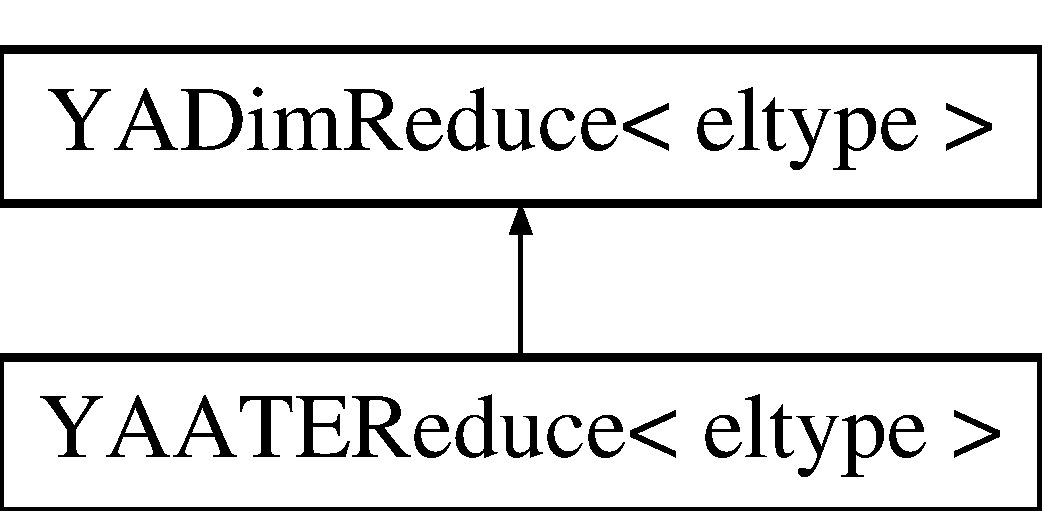
\includegraphics[height=2cm]{class_y_a_a_t_e_reduce}
\end{center}
\end{figure}
\subsection*{Public Member Functions}
\begin{CompactItemize}
\item 
\hypertarget{class_y_a_a_t_e_reduce_a1}{
const string \hyperlink{class_y_a_a_t_e_reduce_a1}{method\_\-name} () const }
\label{class_y_a_a_t_e_reduce_a1}

\begin{CompactList}\small\item\em Return the name of the dimensionality reduction method. \item\end{CompactList}\item 
\hypertarget{class_y_a_a_t_e_reduce_a2}{
const string \hyperlink{class_y_a_a_t_e_reduce_a2}{method\_\-id} () const }
\label{class_y_a_a_t_e_reduce_a2}

\begin{CompactList}\small\item\em Return the id of the dimensionality reduction method. \item\end{CompactList}\item 
\hypertarget{class_y_a_a_t_e_reduce_a3}{
const string \hyperlink{class_y_a_a_t_e_reduce_a3}{version} () const }
\label{class_y_a_a_t_e_reduce_a3}

\begin{CompactList}\small\item\em Return the version of the dimensionality reduction method. \item\end{CompactList}\item 
\hypertarget{class_y_a_a_t_e_reduce_a4}{
void \hyperlink{class_y_a_a_t_e_reduce_a4}{set\_\-rng} (Math\-Random$<$ Math\-Mersenne\-Twister $>$ $\ast$\_\-rng)}
\label{class_y_a_a_t_e_reduce_a4}

\begin{CompactList}\small\item\em Set the random number generator to be used during training. \item\end{CompactList}\item 
int \hyperlink{class_y_a_a_t_e_reduce_a5}{find} (const YA\_\-Mat\-T \&input, YA\_\-Mat\-T \&output, ya\_\-sizet dim, Eigen\-Options \&eigopts)
\begin{CompactList}\small\item\em Find the map for reduction based on initial samples. \item\end{CompactList}\item 
int \hyperlink{class_y_a_a_t_e_reduce_a6}{find} (const YA\_\-Mat\-T \&input, YA\_\-Mat\-T \&test, YA\_\-Mat\-T \&output, ya\_\-sizet dim, Eigen\-Options \&eigopts)
\begin{CompactList}\small\item\em Find the map for reduction based on initial samples with specific test. \item\end{CompactList}\item 
\hypertarget{class_y_a_a_t_e_reduce_a7}{
void \hyperlink{class_y_a_a_t_e_reduce_a7}{forward} (const YA\_\-Mat\-T \&input, YA\_\-Mat\-T \&output) const }
\label{class_y_a_a_t_e_reduce_a7}

\begin{CompactList}\small\item\em Map in the forward direction to reduce the dimensionality of a matrix. \item\end{CompactList}\item 
\hypertarget{class_y_a_a_t_e_reduce_a8}{
void \hyperlink{class_y_a_a_t_e_reduce_a8}{reverse} (const YA\_\-Mat\-T \&input, YA\_\-Mat\-T \&output) const }
\label{class_y_a_a_t_e_reduce_a8}

\begin{CompactList}\small\item\em Map in the reverse direction to increase the dimensionality of a matrix. \item\end{CompactList}\item 
\hypertarget{class_y_a_a_t_e_reduce_a9}{
void \hyperlink{class_y_a_a_t_e_reduce_a9}{save\_\-map} (ostream \&out) const }
\label{class_y_a_a_t_e_reduce_a9}

\begin{CompactList}\small\item\em Save a map to the given stream. \item\end{CompactList}\item 
\hypertarget{class_y_a_a_t_e_reduce_a10}{
int \hyperlink{class_y_a_a_t_e_reduce_a10}{load\_\-map} (istream \&in)}
\label{class_y_a_a_t_e_reduce_a10}

\begin{CompactList}\small\item\em Load a map from the given stream. \item\end{CompactList}\item 
template$<$class vm\_\-type, class ya\_\-type2, class ya\_\-type3, class ya\_\-type4$>$ void \hyperlink{class_y_a_a_t_e_reduce_a11}{train} (const vm\_\-type \&all\_\-data, const ya\_\-type2 \&layers, ya\_\-type3 \&RBM\_\-error, ya\_\-type4 \&BP\_\-error)
\begin{CompactList}\small\item\em Train the Auto\-Encoder using a random split of the data into train/test. \item\end{CompactList}\item 
template$<$class vm\_\-type, class ya\_\-type2, class ya\_\-type3, class ya\_\-type4, class vm\_\-type5$>$ void \hyperlink{class_y_a_a_t_e_reduce_a12}{train} (const vm\_\-type \&train\_\-data, const ya\_\-type2 \&test\_\-data, const ya\_\-type3 \&layers, ya\_\-type4 \&RBM\_\-error, vm\_\-type5 \&BP\_\-error)
\begin{CompactList}\small\item\em Train the Auto\-Encoder using specified training and testing data. \item\end{CompactList}\item 
template$<$class vm\_\-type, class ya\_\-type2, class ya\_\-type3, class ya\_\-type4, class vm\_\-type5$>$ void \hyperlink{class_y_a_a_t_e_reduce_a13}{train} (const vm\_\-type \&train\_\-data, const ya\_\-type2 \&test\_\-data, const ya\_\-type3 \&layers, const YA\_\-Mat$<$ \hyperlink{struct_y_a_a_t_e_reduce_1_1conv__parms}{conv\_\-parms} $>$ \&epsilon, ya\_\-type4 \&RBM\_\-error, vm\_\-type5 \&BP\_\-error)
\begin{CompactList}\small\item\em Train the Auto\-Encoder using specified training/testing data and epsilon. \item\end{CompactList}\item 
template$<$class vm\_\-type, class ya\_\-type2$>$ void \hyperlink{class_y_a_a_t_e_reduce_a14}{forward\_\-map} (const vm\_\-type \&input, ya\_\-type2 \&output) const 
\begin{CompactList}\small\item\em Forward map. \item\end{CompactList}\item 
template$<$class vm\_\-type, class ya\_\-type2$>$ void \hyperlink{class_y_a_a_t_e_reduce_a15}{reverse\_\-map} (const vm\_\-type \&input, ya\_\-type2 \&output) const 
\begin{CompactList}\small\item\em Inverse map. \item\end{CompactList}\item 
\hypertarget{class_y_a_a_t_e_reduce_a16}{
double \hyperlink{class_y_a_a_t_e_reduce_a16}{train\_\-split} () const }
\label{class_y_a_a_t_e_reduce_a16}

\begin{CompactList}\small\item\em percentage of data set that will become training set \item\end{CompactList}\item 
\hypertarget{class_y_a_a_t_e_reduce_a17}{
void \hyperlink{class_y_a_a_t_e_reduce_a17}{train\_\-split} (double i)}
\label{class_y_a_a_t_e_reduce_a17}

\begin{CompactList}\small\item\em set percentage of data set that will become training set \item\end{CompactList}\item 
\hypertarget{class_y_a_a_t_e_reduce_a18}{
ya\_\-sizet \hyperlink{class_y_a_a_t_e_reduce_a18}{rbm\_\-iters} () const }
\label{class_y_a_a_t_e_reduce_a18}

\begin{CompactList}\small\item\em number of iterations for RBM training \item\end{CompactList}\item 
\hypertarget{class_y_a_a_t_e_reduce_a19}{
void \hyperlink{class_y_a_a_t_e_reduce_a19}{rbm\_\-iters} (ya\_\-sizet i)}
\label{class_y_a_a_t_e_reduce_a19}

\begin{CompactList}\small\item\em set number of iterations for RBM training \item\end{CompactList}\item 
\hypertarget{class_y_a_a_t_e_reduce_a20}{
ya\_\-sizet \hyperlink{class_y_a_a_t_e_reduce_a20}{bp\_\-iters} () const }
\label{class_y_a_a_t_e_reduce_a20}

\begin{CompactList}\small\item\em number of iterations for back propagation training \item\end{CompactList}\item 
\hypertarget{class_y_a_a_t_e_reduce_a21}{
void \hyperlink{class_y_a_a_t_e_reduce_a21}{bp\_\-iters} (ya\_\-sizet i)}
\label{class_y_a_a_t_e_reduce_a21}

\begin{CompactList}\small\item\em set number of iterations for back propagation training \item\end{CompactList}\item 
\hypertarget{class_y_a_a_t_e_reduce_a22}{
ya\_\-sizet \hyperlink{class_y_a_a_t_e_reduce_a22}{rbm\_\-size} () const }
\label{class_y_a_a_t_e_reduce_a22}

\begin{CompactList}\small\item\em desired batch sizes for RBM training \item\end{CompactList}\item 
\hypertarget{class_y_a_a_t_e_reduce_a23}{
void \hyperlink{class_y_a_a_t_e_reduce_a23}{rbm\_\-size} (ya\_\-sizet i)}
\label{class_y_a_a_t_e_reduce_a23}

\begin{CompactList}\small\item\em set desired batch sizes for RBM training \item\end{CompactList}\item 
\hypertarget{class_y_a_a_t_e_reduce_a24}{
ya\_\-sizet \hyperlink{class_y_a_a_t_e_reduce_a24}{bp\_\-size} () const }
\label{class_y_a_a_t_e_reduce_a24}

\begin{CompactList}\small\item\em desired batch sizes for BP training \item\end{CompactList}\item 
\hypertarget{class_y_a_a_t_e_reduce_a25}{
void \hyperlink{class_y_a_a_t_e_reduce_a25}{bp\_\-size} (ya\_\-sizet i)}
\label{class_y_a_a_t_e_reduce_a25}

\begin{CompactList}\small\item\em set desired batch sizes for BP training \item\end{CompactList}\item 
\hypertarget{class_y_a_a_t_e_reduce_a26}{
const string \hyperlink{class_y_a_a_t_e_reduce_a26}{logistic\_\-conv} () const }
\label{class_y_a_a_t_e_reduce_a26}

\begin{CompactList}\small\item\em RBM optimization parameters for logistic and linear units. \item\end{CompactList}\item 
\hypertarget{class_y_a_a_t_e_reduce_a27}{
const string \hyperlink{class_y_a_a_t_e_reduce_a27}{logistic\_\-momentum} () const }
\label{class_y_a_a_t_e_reduce_a27}

\begin{CompactList}\small\item\em RBM optimization parameters for logistic and linear units. \item\end{CompactList}\item 
\hypertarget{class_y_a_a_t_e_reduce_a28}{
const string \hyperlink{class_y_a_a_t_e_reduce_a28}{linear\_\-conv} () const }
\label{class_y_a_a_t_e_reduce_a28}

\begin{CompactList}\small\item\em RBM optimization parameters for logistic and linear units. \item\end{CompactList}\item 
\hypertarget{class_y_a_a_t_e_reduce_a29}{
const string \hyperlink{class_y_a_a_t_e_reduce_a29}{linear\_\-momentum} () const }
\label{class_y_a_a_t_e_reduce_a29}

\begin{CompactList}\small\item\em RBM optimization parameters for logistic and linear units. \item\end{CompactList}\item 
double \hyperlink{class_y_a_a_t_e_reduce_a30}{momentum\_\-denom} () const 
\begin{CompactList}\small\item\em optimization default for RBM (when to switch from initial to final momentum) \item\end{CompactList}\item 
ya\_\-sizet \hyperlink{class_y_a_a_t_e_reduce_a31}{num\_\-ls} () const 
\begin{CompactList}\small\item\em number of line searches for conjugate gradient optimization (see minimize) \item\end{CompactList}\item 
\hypertarget{class_y_a_a_t_e_reduce_a32}{
eltype \hyperlink{class_y_a_a_t_e_reduce_a32}{CG\_\-EPS} () const }
\label{class_y_a_a_t_e_reduce_a32}

\begin{CompactList}\small\item\em numerical constants for minimizer \item\end{CompactList}\item 
\hypertarget{class_y_a_a_t_e_reduce_a33}{
eltype \hyperlink{class_y_a_a_t_e_reduce_a33}{CG\_\-REALMIN} () const }
\label{class_y_a_a_t_e_reduce_a33}

\begin{CompactList}\small\item\em numerical constants for minimizer \item\end{CompactList}\item 
\hypertarget{class_y_a_a_t_e_reduce_a34}{
eltype \hyperlink{class_y_a_a_t_e_reduce_a34}{cg\_\-int} () const }
\label{class_y_a_a_t_e_reduce_a34}

\begin{CompactList}\small\item\em don't reevaluate within 0.1 of the limit of the current bracket \item\end{CompactList}\item 
\hypertarget{class_y_a_a_t_e_reduce_a35}{
eltype \hyperlink{class_y_a_a_t_e_reduce_a35}{cg\_\-ext} () const }
\label{class_y_a_a_t_e_reduce_a35}

\begin{CompactList}\small\item\em extrapolate maximum 3 times the current step-size \item\end{CompactList}\item 
\hypertarget{class_y_a_a_t_e_reduce_a36}{
ya\_\-sizet \hyperlink{class_y_a_a_t_e_reduce_a36}{cg\_\-max} () const }
\label{class_y_a_a_t_e_reduce_a36}

\begin{CompactList}\small\item\em maximum number of function evaluations per iteration for CG routine \item\end{CompactList}\item 
\hypertarget{class_y_a_a_t_e_reduce_a37}{
eltype \hyperlink{class_y_a_a_t_e_reduce_a37}{cg\_\-ratio} () const }
\label{class_y_a_a_t_e_reduce_a37}

\begin{CompactList}\small\item\em maximum allowed slope ratio \item\end{CompactList}\item 
eltype \hyperlink{class_y_a_a_t_e_reduce_a38}{cg\_\-sig} () const 
\begin{CompactList}\small\item\em SIG and RHO are the constants controlling the Wolfe-Powell conditions. \item\end{CompactList}\item 
eltype \hyperlink{class_y_a_a_t_e_reduce_a39}{cg\_\-rho} () const 
\begin{CompactList}\small\item\em SIG and RHO are the constants controlling the Wolfe-Powell conditions. \item\end{CompactList}\end{CompactItemize}


\subsection{Detailed Description}
\subsubsection*{template$<$class eltype$>$ class YAATEReduce$<$ eltype $>$}

Dimensionality Reduction via the Auto\-Encoder. 

Autoencoder Formulation in C++ ------------------------------

This implements an autoencoder for dimensionality reduction as described in:

\begin{itemize}
\item Hinton, G.E., and R.R. Salakhutdinov (2006). \char`\"{}Reducing the dimensionality of data with neural networks.\char`\"{} Science 313(5786): 504-507.\end{itemize}


An Auto\-Encoder is given by a sequence of weight matrices, biases and unit functions. These parameters specify the encoder and the decoder which together make up the Auto\-Encoder. An Auto\-Encoder is specified by a sequence of integers n1-n2-n3-...-nd, where n1 is the input dimension, and n2-n3-...-nd are the dimensions of the intermediate maps, with nd representing the final (low dimensional) representation.

Corresponding to the layers of the Auto\-Encoder we have weight matrices W1,...,W(2$\ast$d-2) and biases b1,...,b(2$\ast$d-2). The 1 to d-1 the weight matrices and biases specify the encoder and have dimensions as follows: W1 is n2xn1, b1 is n2x1, W2 is n3xn2, b2 is n3x1, etc.

The encoder is assumed to have all logistic unit functions of the form 1/(1+exp(-x)) except for one linear unit function mapping n(d-1) -$>$ nd.

If X is the n1 by N data matrix with points as columns then the first step of the forward map is given by (using matlab notation)

1./(1+exp(-W1$\ast$X - repmat(b1,1,N))

The full forward map is given by compositions of these functions, the last being linear of the form W(d-1)$\ast$X(d-1) + repmat(b(d-1),1,N), where W(d-1) and b(d-1) are the d-1 weight matrix and bias vector, respectively, and X(d-1) is the d-1 image of X under the previous logistic maps.

Once we reach the ndxn(d-1) weight matrix W(d-1) and ndx1 bias b(d-1), we switch to the decoder, which is specified as follows: Wd is ndxn(d-1), bd is n(d-1), etc. The decoder doesn't have any linear maps. All maps are of the form

1./(1+exp(-W(d)$\ast$Y - repmat(b(d),1,N)).

The full Auto\-Encoder is the composition of all of the forward and inverse maps. 



\subsection{Member Function Documentation}
\hypertarget{class_y_a_a_t_e_reduce_a39}{
\index{YAATEReduce@{YAATEReduce}!cg_rho@{cg\_\-rho}}
\index{cg_rho@{cg\_\-rho}!YAATEReduce@{YAATEReduce}}
\subsubsection[cg\_\-rho]{\setlength{\rightskip}{0pt plus 5cm}template$<$class eltype$>$ eltype \hyperlink{class_y_a_a_t_e_reduce}{YAATEReduce}$<$ eltype $>$::cg\_\-rho () const\hspace{0.3cm}{\tt  \mbox{[}inline\mbox{]}}}}
\label{class_y_a_a_t_e_reduce_a39}


SIG and RHO are the constants controlling the Wolfe-Powell conditions. 

\begin{Desc}
\item[See also:]\hyperlink{class_y_a_a_t_e_reduce_a38}{cg\_\-sig()} $\ast$ \end{Desc}
\hypertarget{class_y_a_a_t_e_reduce_a38}{
\index{YAATEReduce@{YAATEReduce}!cg_sig@{cg\_\-sig}}
\index{cg_sig@{cg\_\-sig}!YAATEReduce@{YAATEReduce}}
\subsubsection[cg\_\-sig]{\setlength{\rightskip}{0pt plus 5cm}template$<$class eltype$>$ eltype \hyperlink{class_y_a_a_t_e_reduce}{YAATEReduce}$<$ eltype $>$::cg\_\-sig () const\hspace{0.3cm}{\tt  \mbox{[}inline\mbox{]}}}}
\label{class_y_a_a_t_e_reduce_a38}


SIG and RHO are the constants controlling the Wolfe-Powell conditions. 

SIG is the maximum allowed absolute ratio between previous and new slopes (derivatives in the search direction), thus setting SIG to low (positive) values forces higher precision in the line-searches. RHO is the minimum allowed fraction of the expected (from the slope at the initial point in the linesearch). Constants must satisfy 0 $<$ RHO $<$ SIG $<$ 1. Tuning of SIG (depending on the nature of the function to be optimized) may speed up the minimization; it is probably not worth playing much with RHO. $\ast$ \hypertarget{class_y_a_a_t_e_reduce_a6}{
\index{YAATEReduce@{YAATEReduce}!find@{find}}
\index{find@{find}!YAATEReduce@{YAATEReduce}}
\subsubsection[find]{\setlength{\rightskip}{0pt plus 5cm}template$<$class eltype$>$ int \hyperlink{class_y_a_a_t_e_reduce}{YAATEReduce}$<$ eltype $>$::find (const YA\_\-Mat\-T \& {\em input}, YA\_\-Mat\-T \& {\em test}, YA\_\-Mat\-T \& {\em output}, ya\_\-sizet {\em dim}, Eigen\-Options \& {\em eigopts})\hspace{0.3cm}{\tt  \mbox{[}inline\mbox{]}}}}
\label{class_y_a_a_t_e_reduce_a6}


Find the map for reduction based on initial samples with specific test. 

\begin{Desc}
\item[Parameters:]
\begin{description}
\item[{\em input}]Train Matrix of initial samples (columns are dimensions) \item[{\em test}]Test Matrix \item[{\em output}]Matrix storing low-dimensioal coords of samples \item[{\em dim}]New dimensionality for output matrix $\ast$ \end{description}
\end{Desc}
\hypertarget{class_y_a_a_t_e_reduce_a5}{
\index{YAATEReduce@{YAATEReduce}!find@{find}}
\index{find@{find}!YAATEReduce@{YAATEReduce}}
\subsubsection[find]{\setlength{\rightskip}{0pt plus 5cm}template$<$class eltype$>$ int \hyperlink{class_y_a_a_t_e_reduce}{YAATEReduce}$<$ eltype $>$::find (const YA\_\-Mat\-T \& {\em input}, YA\_\-Mat\-T \& {\em output}, ya\_\-sizet {\em dim}, Eigen\-Options \& {\em eigopts})\hspace{0.3cm}{\tt  \mbox{[}inline, virtual\mbox{]}}}}
\label{class_y_a_a_t_e_reduce_a5}


Find the map for reduction based on initial samples. 

\begin{Desc}
\item[Parameters:]
\begin{description}
\item[{\em input}]Matrix storing initial samples (columns are dimensions) \item[{\em output}]Matrix storing low-dimensioal coords of samples \item[{\em dim}]New dimensionality for output matrix $\ast$ \end{description}
\end{Desc}


Implements \hyperlink{class_y_a_dim_reduce_a8}{YADim\-Reduce$<$ eltype $>$}.\hypertarget{class_y_a_a_t_e_reduce_a14}{
\index{YAATEReduce@{YAATEReduce}!forward_map@{forward\_\-map}}
\index{forward_map@{forward\_\-map}!YAATEReduce@{YAATEReduce}}
\subsubsection[forward\_\-map]{\setlength{\rightskip}{0pt plus 5cm}template$<$class eltype$>$ template$<$class vm\_\-type, class ya\_\-type2$>$ void \hyperlink{class_y_a_a_t_e_reduce}{YAATEReduce}$<$ eltype $>$::forward\_\-map (const vm\_\-type \& {\em input}, ya\_\-type2 \& {\em output}) const}}
\label{class_y_a_a_t_e_reduce_a14}


Forward map. 

The forward map has all logistic units except for the final map, which is linear. $\ast$ \hypertarget{class_y_a_a_t_e_reduce_a30}{
\index{YAATEReduce@{YAATEReduce}!momentum_denom@{momentum\_\-denom}}
\index{momentum_denom@{momentum\_\-denom}!YAATEReduce@{YAATEReduce}}
\subsubsection[momentum\_\-denom]{\setlength{\rightskip}{0pt plus 5cm}template$<$class eltype$>$ double \hyperlink{class_y_a_a_t_e_reduce}{YAATEReduce}$<$ eltype $>$::momentum\_\-denom () const\hspace{0.3cm}{\tt  \mbox{[}inline\mbox{]}}}}
\label{class_y_a_a_t_e_reduce_a30}


optimization default for RBM (when to switch from initial to final momentum) 

computed as number of iterations/MOMENTUM\_\-DENOM $\ast$ \hypertarget{class_y_a_a_t_e_reduce_a31}{
\index{YAATEReduce@{YAATEReduce}!num_ls@{num\_\-ls}}
\index{num_ls@{num\_\-ls}!YAATEReduce@{YAATEReduce}}
\subsubsection[num\_\-ls]{\setlength{\rightskip}{0pt plus 5cm}template$<$class eltype$>$ ya\_\-sizet \hyperlink{class_y_a_a_t_e_reduce}{YAATEReduce}$<$ eltype $>$::num\_\-ls () const\hspace{0.3cm}{\tt  \mbox{[}inline\mbox{]}}}}
\label{class_y_a_a_t_e_reduce_a31}


number of line searches for conjugate gradient optimization (see minimize) 

\begin{Desc}
\item[Note:]must be $>$ 0. $\ast$ \end{Desc}
\hypertarget{class_y_a_a_t_e_reduce_a15}{
\index{YAATEReduce@{YAATEReduce}!reverse_map@{reverse\_\-map}}
\index{reverse_map@{reverse\_\-map}!YAATEReduce@{YAATEReduce}}
\subsubsection[reverse\_\-map]{\setlength{\rightskip}{0pt plus 5cm}template$<$class eltype$>$ template$<$class vm\_\-type, class ya\_\-type2$>$ void \hyperlink{class_y_a_a_t_e_reduce}{YAATEReduce}$<$ eltype $>$::reverse\_\-map (const vm\_\-type \& {\em input}, ya\_\-type2 \& {\em output}) const}}
\label{class_y_a_a_t_e_reduce_a15}


Inverse map. 

The inverse map has all logistic units. $\ast$ \hypertarget{class_y_a_a_t_e_reduce_a13}{
\index{YAATEReduce@{YAATEReduce}!train@{train}}
\index{train@{train}!YAATEReduce@{YAATEReduce}}
\subsubsection[train]{\setlength{\rightskip}{0pt plus 5cm}template$<$class eltype$>$ template$<$class vm\_\-type, class ya\_\-type2, class ya\_\-type3, class ya\_\-type4, class vm\_\-type5$>$ void \hyperlink{class_y_a_a_t_e_reduce}{YAATEReduce}$<$ eltype $>$::train (const vm\_\-type \& {\em train\_\-data}, const ya\_\-type2 \& {\em test\_\-data}, const ya\_\-type3 \& {\em layers}, const YA\_\-Mat$<$ \hyperlink{struct_y_a_a_t_e_reduce_1_1conv__parms}{conv\_\-parms} $>$ \& {\em epsilon}, ya\_\-type4 \& {\em RBM\_\-error}, vm\_\-type5 \& {\em BP\_\-error})}}
\label{class_y_a_a_t_e_reduce_a13}


Train the Auto\-Encoder using specified training/testing data and epsilon. 

\begin{Desc}
\item[See also:]\hyperlink{class_y_a_a_t_e_reduce_a11}{train()} $\ast$ \end{Desc}
\hypertarget{class_y_a_a_t_e_reduce_a12}{
\index{YAATEReduce@{YAATEReduce}!train@{train}}
\index{train@{train}!YAATEReduce@{YAATEReduce}}
\subsubsection[train]{\setlength{\rightskip}{0pt plus 5cm}template$<$class eltype$>$ template$<$class vm\_\-type, class ya\_\-type2, class ya\_\-type3, class ya\_\-type4, class vm\_\-type5$>$ void \hyperlink{class_y_a_a_t_e_reduce}{YAATEReduce}$<$ eltype $>$::train (const vm\_\-type \& {\em train\_\-data}, const ya\_\-type2 \& {\em test\_\-data}, const ya\_\-type3 \& {\em layers}, ya\_\-type4 \& {\em RBM\_\-error}, vm\_\-type5 \& {\em BP\_\-error})}}
\label{class_y_a_a_t_e_reduce_a12}


Train the Auto\-Encoder using specified training and testing data. 

\begin{Desc}
\item[See also:]\hyperlink{class_y_a_a_t_e_reduce_a11}{train()} $\ast$ \end{Desc}
\hypertarget{class_y_a_a_t_e_reduce_a11}{
\index{YAATEReduce@{YAATEReduce}!train@{train}}
\index{train@{train}!YAATEReduce@{YAATEReduce}}
\subsubsection[train]{\setlength{\rightskip}{0pt plus 5cm}template$<$class eltype$>$ template$<$class vm\_\-type, class ya\_\-type2, class ya\_\-type3, class ya\_\-type4$>$ void \hyperlink{class_y_a_a_t_e_reduce}{YAATEReduce}$<$ eltype $>$::train (const vm\_\-type \& {\em all\_\-data}, const ya\_\-type2 \& {\em layers}, ya\_\-type3 \& {\em RBM\_\-error}, ya\_\-type4 \& {\em BP\_\-error})}}
\label{class_y_a_a_t_e_reduce_a11}


Train the Auto\-Encoder using a random split of the data into train/test. 

The data is split based on \hyperlink{class_y_a_a_t_e_reduce_a16}{train\_\-split()}. \begin{Desc}
\item[Parameters:]
\begin{description}
\item[{\em all\_\-data}]data to be used for training and testing \item[{\em layers}]dimensionality of each layer to be used for mapping \item[{\em RBM\_\-error}]RBM Training Error. Rows are layers, columns iterations \item[{\em BP\_\-error}]BP Training Error. First row is train, second row test \end{description}
\end{Desc}


The documentation for this class was generated from the following files:\begin{CompactItemize}
\item 
/tmp/drl/cpp/math/dimred/ya\_\-ate\_\-reduce.h\item 
/tmp/drl/cpp/math/dimred/ya\_\-ate\_\-reduce.cpp\end{CompactItemize}

\hypertarget{struct_y_a_a_t_e_reduce_1_1conv__parms}{
\section{YAATEReduce$<$ eltype $>$::conv\_\-parms Struct Reference}
\label{struct_y_a_a_t_e_reduce_1_1conv__parms}\index{YAATEReduce::conv_parms@{YAATEReduce::conv\_\-parms}}
}
This structure contains convergence parameters for the 1-step constrastive.  


{\tt \#include $<$ya\_\-ate\_\-reduce.h$>$}

\subsection*{Public Attributes}
\begin{CompactItemize}
\item 
\hypertarget{struct_y_a_a_t_e_reduce_1_1conv__parms_o0}{
YA\_\-Row\-T {\bf conv}}
\label{struct_y_a_a_t_e_reduce_1_1conv__parms_o0}

\item 
\hypertarget{struct_y_a_a_t_e_reduce_1_1conv__parms_o1}{
YA\_\-Row\-T {\bf momentum}}
\label{struct_y_a_a_t_e_reduce_1_1conv__parms_o1}

\end{CompactItemize}


\subsection{Detailed Description}
\subsubsection*{template$<$class eltype$>$ struct YAATEReduce$<$ eltype $>$::conv\_\-parms}

This structure contains convergence parameters for the 1-step constrastive. 

divergence algorithm used to train the Restricted Boltzmann Machines (see train\_\-RBM). $\ast$ 



The documentation for this struct was generated from the following file:\begin{CompactItemize}
\item 
/tmp/drl/cpp/math/dimred/ya\_\-ate\_\-reduce.h\end{CompactItemize}

\hypertarget{class_y_a_dim_reduce}{
\section{YADim\-Reduce$<$ eltype $>$ Class Template Reference}
\label{class_y_a_dim_reduce}\index{YADimReduce@{YADimReduce}}
}
General Base Class for Dimensionality Reduction.  


{\tt \#include $<$ya\_\-dim\_\-reduce.h$>$}

Inheritance diagram for YADim\-Reduce$<$ eltype $>$::\begin{figure}[H]
\begin{center}
\leavevmode
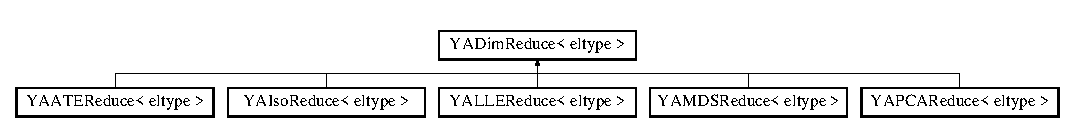
\includegraphics[height=1.34132cm]{class_y_a_dim_reduce}
\end{center}
\end{figure}
\subsection*{Public Member Functions}
\begin{CompactItemize}
\item 
\hypertarget{class_y_a_dim_reduce_a2}{
virtual const string \hyperlink{class_y_a_dim_reduce_a2}{method\_\-name} () const =0}
\label{class_y_a_dim_reduce_a2}

\begin{CompactList}\small\item\em Return the name of the dimensionality reduction method. \item\end{CompactList}\item 
\hypertarget{class_y_a_dim_reduce_a3}{
virtual const string \hyperlink{class_y_a_dim_reduce_a3}{method\_\-id} () const =0}
\label{class_y_a_dim_reduce_a3}

\begin{CompactList}\small\item\em Return the string id of the dimensionality reduction method. \item\end{CompactList}\item 
\hypertarget{class_y_a_dim_reduce_a4}{
virtual const string \hyperlink{class_y_a_dim_reduce_a4}{version} () const =0}
\label{class_y_a_dim_reduce_a4}

\begin{CompactList}\small\item\em Return the version of the dimensionality reduction method. \item\end{CompactList}\item 
template$<$class ya\_\-type1, class ya\_\-type2$>$ int \hyperlink{class_y_a_dim_reduce_a5}{find\_\-t} (const ya\_\-type1 \&input, ya\_\-type2 \&output, ya\_\-sizet dim, Eigen\-Options \&eigopts)
\begin{CompactList}\small\item\em Find the map for reduction based on initial samples. \item\end{CompactList}\item 
\hypertarget{class_y_a_dim_reduce_a6}{
template$<$class ya\_\-type1, class ya\_\-type2$>$ void \hyperlink{class_y_a_dim_reduce_a6}{forward\_\-t} (const ya\_\-type1 \&input, ya\_\-type2 \&output) const }
\label{class_y_a_dim_reduce_a6}

\begin{CompactList}\small\item\em Map in the forward direction to reduce the dimensionality of a matrix. \item\end{CompactList}\item 
\hypertarget{class_y_a_dim_reduce_a7}{
template$<$class ya\_\-type1, class ya\_\-type2$>$ void \hyperlink{class_y_a_dim_reduce_a7}{reverse\_\-t} (const ya\_\-type1 \&input, ya\_\-type2 \&output) const }
\label{class_y_a_dim_reduce_a7}

\begin{CompactList}\small\item\em Map in the reverse direction to increase the dimensionality of a matrix. \item\end{CompactList}\item 
virtual int \hyperlink{class_y_a_dim_reduce_a8}{find} (const YA\_\-Mat\-T \&input, YA\_\-Mat\-T \&output, ya\_\-sizet dim, Eigen\-Options \&eigopts)=0
\begin{CompactList}\small\item\em Find the map for reduction based on initial samples. \item\end{CompactList}\item 
\hypertarget{class_y_a_dim_reduce_a9}{
virtual void \hyperlink{class_y_a_dim_reduce_a9}{forward} (const YA\_\-Mat\-T \&input, YA\_\-Mat\-T \&output) const =0}
\label{class_y_a_dim_reduce_a9}

\begin{CompactList}\small\item\em Map in the forward direction to reduce the dimensionality of a matrix. \item\end{CompactList}\item 
\hypertarget{class_y_a_dim_reduce_a10}{
virtual void \hyperlink{class_y_a_dim_reduce_a10}{reverse} (const YA\_\-Mat\-T \&input, YA\_\-Mat\-T \&output) const =0}
\label{class_y_a_dim_reduce_a10}

\begin{CompactList}\small\item\em Map in the reverse direction to increase the dimensionality of a matrix. \item\end{CompactList}\item 
template$<$class ya\_\-type1$>$ eltype \hyperlink{class_y_a_dim_reduce_a11}{reconstruct\_\-error} (const ya\_\-type1 \&input) const 
\begin{CompactList}\small\item\em RMSD representing the reconstruction error from the input matrix. \item\end{CompactList}\item 
\hypertarget{class_y_a_dim_reduce_a12}{
int \hyperlink{class_y_a_dim_reduce_a12}{save\_\-map} (const string filename) const }
\label{class_y_a_dim_reduce_a12}

\begin{CompactList}\small\item\em Save dimensionality reduction map to the given file name. \item\end{CompactList}\item 
\hypertarget{class_y_a_dim_reduce_a13}{
virtual void \hyperlink{class_y_a_dim_reduce_a13}{save\_\-map} (ostream \&out) const =0}
\label{class_y_a_dim_reduce_a13}

\begin{CompactList}\small\item\em Save dimensionality reduction map to the given stream. \item\end{CompactList}\item 
int \hyperlink{class_y_a_dim_reduce_a14}{load\_\-map} (const string filename)
\begin{CompactList}\small\item\em Load dimensionality reduction maps from the given file name. \item\end{CompactList}\item 
\hypertarget{class_y_a_dim_reduce_a15}{
virtual int \hyperlink{class_y_a_dim_reduce_a15}{load\_\-map} (istream \&in)=0}
\label{class_y_a_dim_reduce_a15}

\begin{CompactList}\small\item\em Save a map from the given stream. \item\end{CompactList}\item 
int \hyperlink{class_y_a_dim_reduce_a16}{verbose} ()
\begin{CompactList}\small\item\em Return the degree of output to console by routines. \item\end{CompactList}\item 
void \hyperlink{class_y_a_dim_reduce_a17}{verbose} (const int v)
\begin{CompactList}\small\item\em Set the degree of output to console by routines. \item\end{CompactList}\item 
\hypertarget{class_y_a_dim_reduce_a18}{
ya\_\-sizet \hyperlink{class_y_a_dim_reduce_a18}{high\_\-dim} () const }
\label{class_y_a_dim_reduce_a18}

\begin{CompactList}\small\item\em Return the dimensionality for the high dimensional space. \item\end{CompactList}\item 
\hypertarget{class_y_a_dim_reduce_a19}{
ya\_\-sizet \hyperlink{class_y_a_dim_reduce_a19}{low\_\-dim} () const }
\label{class_y_a_dim_reduce_a19}

\begin{CompactList}\small\item\em Return the dimensionality for the low dimensional space. \item\end{CompactList}\item 
\hypertarget{class_y_a_dim_reduce_a20}{
const YA\_\-Vec\-T \& \hyperlink{class_y_a_dim_reduce_a20}{eigenvalues} () const }
\label{class_y_a_dim_reduce_a20}

\begin{CompactList}\small\item\em Return the vector of eigen values obtained for map. \item\end{CompactList}\item 
\hypertarget{class_y_a_dim_reduce_a21}{
ya\_\-sizet \hyperlink{class_y_a_dim_reduce_a21}{neighbors} () const }
\label{class_y_a_dim_reduce_a21}

\begin{CompactList}\small\item\em Get the number of neighbors for LLE and Iso\-Map. \item\end{CompactList}\item 
\hypertarget{class_y_a_dim_reduce_a22}{
void \hyperlink{class_y_a_dim_reduce_a22}{neighbors} (ya\_\-sizet n)}
\label{class_y_a_dim_reduce_a22}

\begin{CompactList}\small\item\em Set the number of neighbors for LLE and Iso\-Map and use nearest neighbors. \item\end{CompactList}\item 
\hypertarget{class_y_a_dim_reduce_a23}{
eltype \hyperlink{class_y_a_dim_reduce_a23}{epsilon} () const }
\label{class_y_a_dim_reduce_a23}

\begin{CompactList}\small\item\em Get the number of neighbors for LLE and Iso\-Map. \item\end{CompactList}\item 
\hypertarget{class_y_a_dim_reduce_a24}{
void \hyperlink{class_y_a_dim_reduce_a24}{epsilon} (eltype n)}
\label{class_y_a_dim_reduce_a24}

\begin{CompactList}\small\item\em Set the number of neighbors for LLE and Iso\-Map and use epsilon. \item\end{CompactList}\item 
ya\_\-sizet \hyperlink{class_y_a_dim_reduce_a25}{neighbor\_\-mode} () const 
\begin{CompactList}\small\item\em Get the method for obtaining neighbors for LLE and Iso\-Map. \item\end{CompactList}\item 
void \hyperlink{class_y_a_dim_reduce_a26}{neighbor\_\-mode} (ya\_\-sizet n)
\begin{CompactList}\small\item\em Set the method for obtaining neighbors for LLE and Iso\-Map. \item\end{CompactList}\item 
ya\_\-sizet \hyperlink{class_y_a_dim_reduce_a27}{neighbor\_\-weight\_\-mode} () const 
\begin{CompactList}\small\item\em Get the method for obtaining weights in nbors\_\-forward/nbors\_\-reverse. \item\end{CompactList}\item 
void \hyperlink{class_y_a_dim_reduce_a28}{neighbor\_\-weight\_\-mode} (const ya\_\-sizet t)
\begin{CompactList}\small\item\em Set the method for obtaining weights in nbors\_\-forward/nbors\_\-reverse. \item\end{CompactList}\item 
\hypertarget{class_y_a_dim_reduce_a29}{
template$<$class vm\_\-type$>$ void \hyperlink{class_y_a_dim_reduce_a29}{ae\_\-layers} (const vm\_\-type \&in)}
\label{class_y_a_dim_reduce_a29}

\begin{CompactList}\small\item\em Set the dimensionalities of the layers for the Auto\-Encoder. \item\end{CompactList}\item 
\hypertarget{class_y_a_dim_reduce_a30}{
const YA\_\-Mat\-T \& \hyperlink{class_y_a_dim_reduce_a30}{rbm\_\-errors} () const }
\label{class_y_a_dim_reduce_a30}

\begin{CompactList}\small\item\em Get the RBM errors from Auto\-Encoder training. \item\end{CompactList}\item 
\hypertarget{class_y_a_dim_reduce_a31}{
const YA\_\-Mat\-T \& \hyperlink{class_y_a_dim_reduce_a31}{bp\_\-errors} () const }
\label{class_y_a_dim_reduce_a31}

\begin{CompactList}\small\item\em Get the BP errors from Auto\-Encoder training. \item\end{CompactList}\item 
template$<$class vm\_\-type, class ya\_\-type2$>$ int \hyperlink{class_y_a_dim_reduce_a32}{nbors\_\-forward} (const vm\_\-type \&in, ya\_\-type2 \&out) const 
\begin{CompactList}\small\item\em Perform forward map as a weighted average of k-neighbors. \item\end{CompactList}\item 
template$<$class vm\_\-type, class ya\_\-type2$>$ int \hyperlink{class_y_a_dim_reduce_a33}{nbors\_\-reverse} (const vm\_\-type \&in, ya\_\-type2 \&out) const 
\begin{CompactList}\small\item\em Perform reverse map as a weighted average of k-neighbors. \item\end{CompactList}\item 
template$<$class vm\_\-type, class ya\_\-type2$>$ int \hyperlink{class_y_a_dim_reduce_a34}{nbors\_\-forward} (const vm\_\-type \&in, const ya\_\-sizet dim, ya\_\-type2 \&out) const 
\begin{CompactList}\small\item\em Perform forward map using weighted average to dim smaller than lowdim. \item\end{CompactList}\item 
template$<$class vm\_\-type, class ya\_\-type2$>$ int \hyperlink{class_y_a_dim_reduce_a35}{nbors\_\-reverse} (const vm\_\-type \&in, const ya\_\-sizet dim, ya\_\-type2 \&out) const 
\begin{CompactList}\small\item\em Perform reverse map using weighted average from smaller than lowdim. \item\end{CompactList}\item 
template$<$class mat\_\-type$>$ void \hyperlink{class_y_a_dim_reduce_a36}{double\_\-center} (YA\_\-Base\-T \&mat)
\begin{CompactList}\small\item\em Double center a matrix. \item\end{CompactList}\end{CompactItemize}
\subsection*{Protected Member Functions}
\begin{CompactItemize}
\item 
\hypertarget{class_y_a_dim_reduce_b0}{
template$<$class vm\_\-type, class ya\_\-type2, class ya\_\-type3, class ya\_\-type4$>$ void {\bf lle\_\-weights} (const vm\_\-type \&input, const ya\_\-type2 \&kinput, const ya\_\-sizet k, ya\_\-type3 \&neighbors, ya\_\-type4 \&weights, const bool samemat) const }
\label{class_y_a_dim_reduce_b0}

\item 
\hypertarget{class_y_a_dim_reduce_b1}{
template$<$class vm\_\-type, class ya\_\-type2$>$ void {\bf lle\_\-weightse} (const vm\_\-type \&input, const ya\_\-type2 \&kinput, const eltype epsilon, vector$<$ YA\_\-Dyn\-I $>$ \&neighbors, vector$<$ YA\_\-Dyn\-T $>$ \&weights, const bool samemat) const }
\label{class_y_a_dim_reduce_b1}

\item 
\hypertarget{class_y_a_dim_reduce_b2}{
template$<$class vm\_\-type, class ya\_\-type2, class ya\_\-type3, class ya\_\-type4$>$ void {\bf dist\_\-weights} (const vm\_\-type \&input, const ya\_\-type2 \&kinput, const ya\_\-sizet k, ya\_\-type3 \&neighbors, ya\_\-type4 \&weights) const }
\label{class_y_a_dim_reduce_b2}

\item 
\hypertarget{class_y_a_dim_reduce_b3}{
template$<$class vm\_\-type, class ya\_\-type2$>$ void {\bf dist\_\-weightse} (const vm\_\-type \&input, const ya\_\-type2 \&kinput, const eltype epsilon, vector$<$ YA\_\-Dyn\-I $>$ \&nbors, vector$<$ YA\_\-Dyn\-T $>$ \&weights) const }
\label{class_y_a_dim_reduce_b3}

\item 
\hypertarget{class_y_a_dim_reduce_b4}{
void {\bf write\_\-header} (ostream \&out) const }
\label{class_y_a_dim_reduce_b4}

\item 
\hypertarget{class_y_a_dim_reduce_b5}{
int {\bf read\_\-header} (istream \&in)}
\label{class_y_a_dim_reduce_b5}

\end{CompactItemize}
\subsection*{Protected Attributes}
\begin{CompactItemize}
\item 
\hypertarget{class_y_a_dim_reduce_p0}{
ya\_\-sizet {\bf \_\-high\_\-dim}}
\label{class_y_a_dim_reduce_p0}

\item 
\hypertarget{class_y_a_dim_reduce_p1}{
ya\_\-sizet {\bf \_\-low\_\-dim}}
\label{class_y_a_dim_reduce_p1}

\item 
\hypertarget{class_y_a_dim_reduce_p2}{
YA\_\-Vec\-T {\bf eigen\_\-values}}
\label{class_y_a_dim_reduce_p2}

\item 
\hypertarget{class_y_a_dim_reduce_p3}{
ya\_\-sizet {\bf num\_\-neighbors}}
\label{class_y_a_dim_reduce_p3}

\item 
\hypertarget{class_y_a_dim_reduce_p4}{
eltype {\bf \_\-epsilon}}
\label{class_y_a_dim_reduce_p4}

\item 
\hypertarget{class_y_a_dim_reduce_p5}{
ya\_\-sizet {\bf \_\-neighbor\_\-mode}}
\label{class_y_a_dim_reduce_p5}

\item 
\hypertarget{class_y_a_dim_reduce_p6}{
ya\_\-sizet {\bf \_\-neighbor\_\-weight\_\-mode}}
\label{class_y_a_dim_reduce_p6}

\item 
\hypertarget{class_y_a_dim_reduce_p7}{
YA\_\-Row\-I {\bf ate\_\-layers}}
\label{class_y_a_dim_reduce_p7}

\item 
\hypertarget{class_y_a_dim_reduce_p8}{
YA\_\-Mat\-T {\bf rbm\_\-error}}
\label{class_y_a_dim_reduce_p8}

\item 
\hypertarget{class_y_a_dim_reduce_p9}{
YA\_\-Mat\-T {\bf bp\_\-error}}
\label{class_y_a_dim_reduce_p9}

\item 
\hypertarget{class_y_a_dim_reduce_p10}{
YA\_\-Mat\-T {\bf input\_\-coords}}
\label{class_y_a_dim_reduce_p10}

\item 
\hypertarget{class_y_a_dim_reduce_p11}{
YA\_\-Mat\-T {\bf output\_\-coords}}
\label{class_y_a_dim_reduce_p11}

\item 
\hypertarget{class_y_a_dim_reduce_p12}{
int {\bf \_\-verbose}}
\label{class_y_a_dim_reduce_p12}

\end{CompactItemize}


\subsection{Detailed Description}
\subsubsection*{template$<$class eltype$>$ class YADim\-Reduce$<$ eltype $>$}

General Base Class for Dimensionality Reduction. 



\subsection{Member Function Documentation}
\hypertarget{class_y_a_dim_reduce_a36}{
\index{YADimReduce@{YADim\-Reduce}!double_center@{double\_\-center}}
\index{double_center@{double\_\-center}!YADimReduce@{YADim\-Reduce}}
\subsubsection[double\_\-center]{\setlength{\rightskip}{0pt plus 5cm}template$<$class eltype$>$ template$<$class mat\_\-type$>$ void \hyperlink{class_y_a_dim_reduce}{YADim\-Reduce}$<$ eltype $>$::double\_\-center (YA\_\-Base\-T \& {\em mat})}}
\label{class_y_a_dim_reduce_a36}


Double center a matrix. 

Center the matrix by substracting the mean of each column, row, adding the overall mean, and multiplying by -0.5 $\ast$ \hypertarget{class_y_a_dim_reduce_a8}{
\index{YADimReduce@{YADim\-Reduce}!find@{find}}
\index{find@{find}!YADimReduce@{YADim\-Reduce}}
\subsubsection[find]{\setlength{\rightskip}{0pt plus 5cm}template$<$class eltype$>$ virtual int \hyperlink{class_y_a_dim_reduce}{YADim\-Reduce}$<$ eltype $>$::find (const YA\_\-Mat\-T \& {\em input}, YA\_\-Mat\-T \& {\em output}, ya\_\-sizet {\em dim}, Eigen\-Options \& {\em eigopts})\hspace{0.3cm}{\tt  \mbox{[}pure virtual\mbox{]}}}}
\label{class_y_a_dim_reduce_a8}


Find the map for reduction based on initial samples. 

\begin{Desc}
\item[Parameters:]
\begin{description}
\item[{\em input}]Matrix storing initial samples (columns are dimensions) \item[{\em output}]Matrix storing low-dimensioal mapping of samples \item[{\em dim}]New dimensionality for output matrix $\ast$ \end{description}
\end{Desc}


Implemented in \hyperlink{class_y_a_a_t_e_reduce_a5}{YAATEReduce$<$ eltype $>$}, \hyperlink{class_y_a_iso_reduce_a9}{YAIso\-Reduce$<$ eltype $>$}, \hyperlink{class_y_a_l_l_e_reduce_a8}{YALLEReduce$<$ eltype $>$}, \hyperlink{class_y_a_m_d_s_reduce_a8}{YAMDSReduce$<$ eltype $>$}, and \hyperlink{class_y_a_p_c_a_reduce_a8}{YAPCAReduce$<$ eltype $>$}.\hypertarget{class_y_a_dim_reduce_a5}{
\index{YADimReduce@{YADim\-Reduce}!find_t@{find\_\-t}}
\index{find_t@{find\_\-t}!YADimReduce@{YADim\-Reduce}}
\subsubsection[find\_\-t]{\setlength{\rightskip}{0pt plus 5cm}template$<$class eltype$>$ template$<$class ya\_\-type1, class ya\_\-type2$>$ int \hyperlink{class_y_a_dim_reduce}{YADim\-Reduce}$<$ eltype $>$::find\_\-t (const ya\_\-type1 \& {\em input}, ya\_\-type2 \& {\em output}, ya\_\-sizet {\em dim}, Eigen\-Options \& {\em eigopts})\hspace{0.3cm}{\tt  \mbox{[}inline\mbox{]}}}}
\label{class_y_a_dim_reduce_a5}


Find the map for reduction based on initial samples. 

\begin{Desc}
\item[Parameters:]
\begin{description}
\item[{\em input}]Matrix storing initial samples (columns are dimensions) \item[{\em output}]Matrix storing low-dimensioal mapping of samples \item[{\em dim}]New dimensionality for output matrix $\ast$ \end{description}
\end{Desc}
\hypertarget{class_y_a_dim_reduce_a14}{
\index{YADimReduce@{YADim\-Reduce}!load_map@{load\_\-map}}
\index{load_map@{load\_\-map}!YADimReduce@{YADim\-Reduce}}
\subsubsection[load\_\-map]{\setlength{\rightskip}{0pt plus 5cm}template$<$class eltype$>$ int \hyperlink{class_y_a_dim_reduce}{YADim\-Reduce}$<$ eltype $>$::load\_\-map (const string {\em filename})}}
\label{class_y_a_dim_reduce_a14}


Load dimensionality reduction maps from the given file name. 

Can generate the following errors:\begin{itemize}
\item 310/10 Improperly formatted reduction file\end{itemize}


311/10 Reduction method does not match object type\begin{itemize}
\item 312/4 Version does not match current version $\ast$ \end{itemize}
\hypertarget{class_y_a_dim_reduce_a34}{
\index{YADimReduce@{YADim\-Reduce}!nbors_forward@{nbors\_\-forward}}
\index{nbors_forward@{nbors\_\-forward}!YADimReduce@{YADim\-Reduce}}
\subsubsection[nbors\_\-forward]{\setlength{\rightskip}{0pt plus 5cm}template$<$class eltype$>$ template$<$class vm\_\-type, class ya\_\-type2$>$ int \hyperlink{class_y_a_dim_reduce}{YADim\-Reduce}$<$ eltype $>$::nbors\_\-forward (const vm\_\-type \& {\em in}, const ya\_\-sizet {\em dim}, ya\_\-type2 \& {\em out}) const}}
\label{class_y_a_dim_reduce_a34}


Perform forward map using weighted average to dim smaller than lowdim. 

\begin{Desc}
\item[See also:]\hyperlink{class_y_a_dim_reduce_a32}{nbors\_\-forward} $\ast$ \end{Desc}
\hypertarget{class_y_a_dim_reduce_a32}{
\index{YADimReduce@{YADim\-Reduce}!nbors_forward@{nbors\_\-forward}}
\index{nbors_forward@{nbors\_\-forward}!YADimReduce@{YADim\-Reduce}}
\subsubsection[nbors\_\-forward]{\setlength{\rightskip}{0pt plus 5cm}template$<$class eltype$>$ template$<$class vm\_\-type, class ya\_\-type2$>$ int \hyperlink{class_y_a_dim_reduce}{YADim\-Reduce}$<$ eltype $>$::nbors\_\-forward (const vm\_\-type \& {\em in}, ya\_\-type2 \& {\em out}) const}}
\label{class_y_a_dim_reduce_a32}


Perform forward map as a weighted average of k-neighbors. 

The method used to determine the weights is set by \hyperlink{class_y_a_dim_reduce_a27}{neighbor\_\-weight\_\-mode()} \begin{Desc}
\item[Note:]the number of neighbors used is determined by \hyperlink{class_y_a_dim_reduce_a21}{neighbors()} $\ast$ \end{Desc}
\hypertarget{class_y_a_dim_reduce_a35}{
\index{YADimReduce@{YADim\-Reduce}!nbors_reverse@{nbors\_\-reverse}}
\index{nbors_reverse@{nbors\_\-reverse}!YADimReduce@{YADim\-Reduce}}
\subsubsection[nbors\_\-reverse]{\setlength{\rightskip}{0pt plus 5cm}template$<$class eltype$>$ template$<$class vm\_\-type, class ya\_\-type2$>$ int \hyperlink{class_y_a_dim_reduce}{YADim\-Reduce}$<$ eltype $>$::nbors\_\-reverse (const vm\_\-type \& {\em in}, const ya\_\-sizet {\em dim}, ya\_\-type2 \& {\em out}) const}}
\label{class_y_a_dim_reduce_a35}


Perform reverse map using weighted average from smaller than lowdim. 

\begin{Desc}
\item[See also:]\hyperlink{class_y_a_dim_reduce_a33}{nbors\_\-reverse()} $\ast$ \end{Desc}
\hypertarget{class_y_a_dim_reduce_a33}{
\index{YADimReduce@{YADim\-Reduce}!nbors_reverse@{nbors\_\-reverse}}
\index{nbors_reverse@{nbors\_\-reverse}!YADimReduce@{YADim\-Reduce}}
\subsubsection[nbors\_\-reverse]{\setlength{\rightskip}{0pt plus 5cm}template$<$class eltype$>$ template$<$class vm\_\-type, class ya\_\-type2$>$ int \hyperlink{class_y_a_dim_reduce}{YADim\-Reduce}$<$ eltype $>$::nbors\_\-reverse (const vm\_\-type \& {\em in}, ya\_\-type2 \& {\em out}) const}}
\label{class_y_a_dim_reduce_a33}


Perform reverse map as a weighted average of k-neighbors. 

The method used to determine the weights is set by \hyperlink{class_y_a_dim_reduce_a27}{neighbor\_\-weight\_\-mode()} \begin{Desc}
\item[Note:]the number of neighbors used is determined by \hyperlink{class_y_a_dim_reduce_a21}{neighbors()} $\ast$ \end{Desc}
\hypertarget{class_y_a_dim_reduce_a26}{
\index{YADimReduce@{YADim\-Reduce}!neighbor_mode@{neighbor\_\-mode}}
\index{neighbor_mode@{neighbor\_\-mode}!YADimReduce@{YADim\-Reduce}}
\subsubsection[neighbor\_\-mode]{\setlength{\rightskip}{0pt plus 5cm}template$<$class eltype$>$ void \hyperlink{class_y_a_dim_reduce}{YADim\-Reduce}$<$ eltype $>$::neighbor\_\-mode (ya\_\-sizet {\em n})\hspace{0.3cm}{\tt  \mbox{[}inline\mbox{]}}}}
\label{class_y_a_dim_reduce_a26}


Set the method for obtaining neighbors for LLE and Iso\-Map. 

0 is nearest neighbors and 1 is epsilon The neighbor\_\-mode is automatically set accordingly when using \hyperlink{class_y_a_dim_reduce_a21}{neighbors()} or \hyperlink{class_y_a_dim_reduce_a23}{epsilon()} $\ast$ \hypertarget{class_y_a_dim_reduce_a25}{
\index{YADimReduce@{YADim\-Reduce}!neighbor_mode@{neighbor\_\-mode}}
\index{neighbor_mode@{neighbor\_\-mode}!YADimReduce@{YADim\-Reduce}}
\subsubsection[neighbor\_\-mode]{\setlength{\rightskip}{0pt plus 5cm}template$<$class eltype$>$ ya\_\-sizet \hyperlink{class_y_a_dim_reduce}{YADim\-Reduce}$<$ eltype $>$::neighbor\_\-mode () const\hspace{0.3cm}{\tt  \mbox{[}inline\mbox{]}}}}
\label{class_y_a_dim_reduce_a25}


Get the method for obtaining neighbors for LLE and Iso\-Map. 

0 is nearest neighbors and 1 is epsilon $\ast$ \hypertarget{class_y_a_dim_reduce_a28}{
\index{YADimReduce@{YADim\-Reduce}!neighbor_weight_mode@{neighbor\_\-weight\_\-mode}}
\index{neighbor_weight_mode@{neighbor\_\-weight\_\-mode}!YADimReduce@{YADim\-Reduce}}
\subsubsection[neighbor\_\-weight\_\-mode]{\setlength{\rightskip}{0pt plus 5cm}template$<$class eltype$>$ void \hyperlink{class_y_a_dim_reduce}{YADim\-Reduce}$<$ eltype $>$::neighbor\_\-weight\_\-mode (const ya\_\-sizet {\em t})\hspace{0.3cm}{\tt  \mbox{[}inline\mbox{]}}}}
\label{class_y_a_dim_reduce_a28}


Set the method for obtaining weights in nbors\_\-forward/nbors\_\-reverse. 

\begin{itemize}
\item 0 : The weights are set as 1/distance to each neighbor and scaled to sum to 1\begin{itemize}
\item 1 : A least-squares problem is solved to optimize the weights as is performed in LLE \begin{Desc}
\item[See also:]\hyperlink{class_y_a_dim_reduce_a27}{neighbor\_\-weight\_\-mode()}, \hyperlink{class_y_a_dim_reduce_a32}{nbors\_\-forward()}, \hyperlink{class_y_a_dim_reduce_a33}{nbors\_\-reverse()} $\ast$ \end{Desc}
\end{itemize}
\end{itemize}
\hypertarget{class_y_a_dim_reduce_a27}{
\index{YADimReduce@{YADim\-Reduce}!neighbor_weight_mode@{neighbor\_\-weight\_\-mode}}
\index{neighbor_weight_mode@{neighbor\_\-weight\_\-mode}!YADimReduce@{YADim\-Reduce}}
\subsubsection[neighbor\_\-weight\_\-mode]{\setlength{\rightskip}{0pt plus 5cm}template$<$class eltype$>$ ya\_\-sizet \hyperlink{class_y_a_dim_reduce}{YADim\-Reduce}$<$ eltype $>$::neighbor\_\-weight\_\-mode () const\hspace{0.3cm}{\tt  \mbox{[}inline\mbox{]}}}}
\label{class_y_a_dim_reduce_a27}


Get the method for obtaining weights in nbors\_\-forward/nbors\_\-reverse. 

\begin{Desc}
\item[See also:]\hyperlink{class_y_a_dim_reduce_a27}{neighbor\_\-weight\_\-mode()}, \hyperlink{class_y_a_dim_reduce_a32}{nbors\_\-forward()}, \hyperlink{class_y_a_dim_reduce_a33}{nbors\_\-reverse()} $\ast$ \end{Desc}
\hypertarget{class_y_a_dim_reduce_a11}{
\index{YADimReduce@{YADim\-Reduce}!reconstruct_error@{reconstruct\_\-error}}
\index{reconstruct_error@{reconstruct\_\-error}!YADimReduce@{YADim\-Reduce}}
\subsubsection[reconstruct\_\-error]{\setlength{\rightskip}{0pt plus 5cm}template$<$class eltype$>$ template$<$class ya\_\-type1$>$ eltype \hyperlink{class_y_a_dim_reduce}{YADim\-Reduce}$<$ eltype $>$::reconstruct\_\-error (const ya\_\-type1 \& {\em input}) const}}
\label{class_y_a_dim_reduce_a11}


RMSD representing the reconstruction error from the input matrix. 

This is calculating by applying the forward map follwed by the reverse map. $\ast$ \hypertarget{class_y_a_dim_reduce_a17}{
\index{YADimReduce@{YADim\-Reduce}!verbose@{verbose}}
\index{verbose@{verbose}!YADimReduce@{YADim\-Reduce}}
\subsubsection[verbose]{\setlength{\rightskip}{0pt plus 5cm}template$<$class eltype$>$ void \hyperlink{class_y_a_dim_reduce}{YADim\-Reduce}$<$ eltype $>$::verbose (const int {\em v})\hspace{0.3cm}{\tt  \mbox{[}inline\mbox{]}}}}
\label{class_y_a_dim_reduce_a17}


Set the degree of output to console by routines. 

0 is no output, 1 outputs a progress meter, 2 also output nbor stats $\ast$ \hypertarget{class_y_a_dim_reduce_a16}{
\index{YADimReduce@{YADim\-Reduce}!verbose@{verbose}}
\index{verbose@{verbose}!YADimReduce@{YADim\-Reduce}}
\subsubsection[verbose]{\setlength{\rightskip}{0pt plus 5cm}template$<$class eltype$>$ int \hyperlink{class_y_a_dim_reduce}{YADim\-Reduce}$<$ eltype $>$::verbose ()\hspace{0.3cm}{\tt  \mbox{[}inline\mbox{]}}}}
\label{class_y_a_dim_reduce_a16}


Return the degree of output to console by routines. 

0 is no output, 1 outputs a progress meter, 2 also output nbor stats $\ast$ 

The documentation for this class was generated from the following files:\begin{CompactItemize}
\item 
/tmp/drl/cpp/math/dimred/\hyperlink{ya__dim__reduce_8h}{ya\_\-dim\_\-reduce.h}\item 
/tmp/drl/cpp/math/dimred/ya\_\-dim\_\-reduce.cpp\end{CompactItemize}

\hypertarget{class_y_a_iso_reduce}{
\section{YAIso\-Reduce$<$ eltype $>$ Class Template Reference}
\label{class_y_a_iso_reduce}\index{YAIsoReduce@{YAIsoReduce}}
}
Dimensionality reduction using Iso\-Map.  


{\tt \#include $<$ya\_\-iso\_\-reduce.h$>$}

Inheritance diagram for YAIso\-Reduce$<$ eltype $>$::\begin{figure}[H]
\begin{center}
\leavevmode
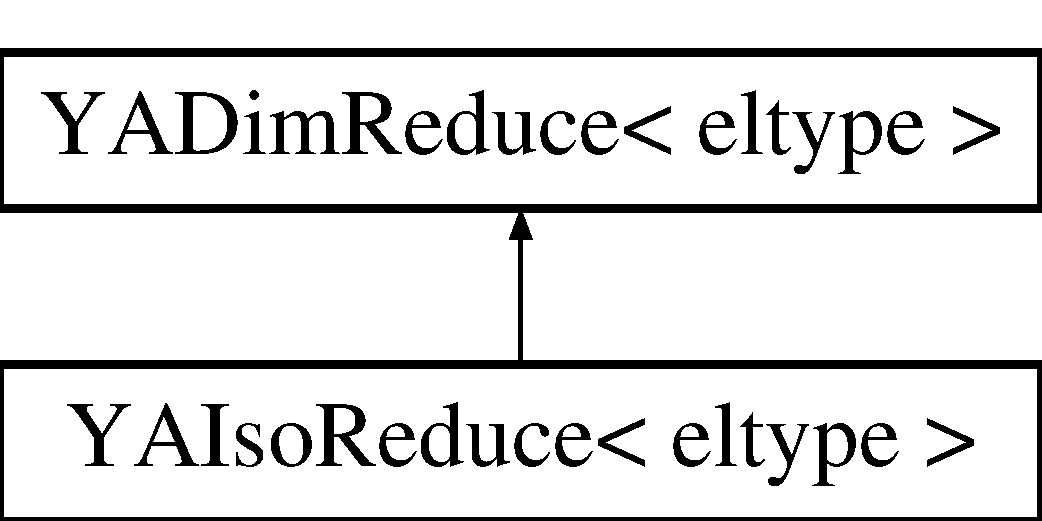
\includegraphics[height=2cm]{class_y_a_iso_reduce}
\end{center}
\end{figure}
\subsection*{Public Member Functions}
\begin{CompactItemize}
\item 
\hypertarget{class_y_a_iso_reduce_a2}{
const string \hyperlink{class_y_a_iso_reduce_a2}{method\_\-name} () const }
\label{class_y_a_iso_reduce_a2}

\begin{CompactList}\small\item\em Return the name of the dimensionality reduction method. \item\end{CompactList}\item 
\hypertarget{class_y_a_iso_reduce_a3}{
const string \hyperlink{class_y_a_iso_reduce_a3}{method\_\-id} () const }
\label{class_y_a_iso_reduce_a3}

\begin{CompactList}\small\item\em Return the id of the dimensionality reduction method. \item\end{CompactList}\item 
\hypertarget{class_y_a_iso_reduce_a4}{
const string \hyperlink{class_y_a_iso_reduce_a4}{version} () const }
\label{class_y_a_iso_reduce_a4}

\begin{CompactList}\small\item\em Return the version of the dimensionality reduction method. \item\end{CompactList}\item 
template$<$class ya\_\-type1, class ya\_\-type2$>$ int \hyperlink{class_y_a_iso_reduce_a5}{find\_\-map} (const ya\_\-type1 \&input, ya\_\-type2 \&output, ya\_\-sizet dim, Eigen\-Options \&eigopts)
\begin{CompactList}\small\item\em Find the reduction based on initial samples. \item\end{CompactList}\item 
template$<$class ya\_\-type1, class ya\_\-type2, class ya\_\-type3$>$ int \hyperlink{class_y_a_iso_reduce_a6}{find\_\-map} (const ya\_\-type1 \&input, ya\_\-type2 \&output, ya\_\-sizet dim, Eigen\-Options \&eigopts, ya\_\-type3 \&landmarks)
\begin{CompactList}\small\item\em Find the reduction based on initial samples using landmarks. \item\end{CompactList}\item 
\hypertarget{class_y_a_iso_reduce_a7}{
template$<$class ya\_\-type1, class ya\_\-type2$>$ void \hyperlink{class_y_a_iso_reduce_a7}{forward\_\-map} (const ya\_\-type1 \&input, ya\_\-type2 \&output) const }
\label{class_y_a_iso_reduce_a7}

\begin{CompactList}\small\item\em Map in the forward direction to reduce the dimensionality of a matrix. \item\end{CompactList}\item 
\hypertarget{class_y_a_iso_reduce_a8}{
template$<$class ya\_\-type1, class ya\_\-type2$>$ void \hyperlink{class_y_a_iso_reduce_a8}{reverse\_\-map} (const ya\_\-type1 \&input, ya\_\-type2 \&output) const }
\label{class_y_a_iso_reduce_a8}

\begin{CompactList}\small\item\em Map in the reverse direction to increase the dimensionality of a matrix. \item\end{CompactList}\item 
int \hyperlink{class_y_a_iso_reduce_a9}{find} (const YA\_\-Mat\-T \&input, YA\_\-Mat\-T \&output, ya\_\-sizet dim, Eigen\-Options \&eigopts)
\begin{CompactList}\small\item\em Find the reduction based on initial samples. \item\end{CompactList}\item 
\hypertarget{class_y_a_iso_reduce_a10}{
void \hyperlink{class_y_a_iso_reduce_a10}{forward} (const YA\_\-Mat\-T \&input, YA\_\-Mat\-T \&output) const }
\label{class_y_a_iso_reduce_a10}

\begin{CompactList}\small\item\em Map in the forward direction to reduce the dimensionality of a matrix. \item\end{CompactList}\item 
\hypertarget{class_y_a_iso_reduce_a11}{
void \hyperlink{class_y_a_iso_reduce_a11}{reverse} (const YA\_\-Mat\-T \&input, YA\_\-Mat\-T \&output) const }
\label{class_y_a_iso_reduce_a11}

\begin{CompactList}\small\item\em Map in the reverse direction to increase the dimensionality of a matrix. \item\end{CompactList}\item 
\hypertarget{class_y_a_iso_reduce_a12}{
void \hyperlink{class_y_a_iso_reduce_a12}{save\_\-map} (ostream \&out) const }
\label{class_y_a_iso_reduce_a12}

\begin{CompactList}\small\item\em Save a map to the given stream. \item\end{CompactList}\item 
\hypertarget{class_y_a_iso_reduce_a13}{
int \hyperlink{class_y_a_iso_reduce_a13}{load\_\-map} (istream \&in)}
\label{class_y_a_iso_reduce_a13}

\begin{CompactList}\small\item\em Load a map from the given stream. \item\end{CompactList}\item 
\hypertarget{class_y_a_iso_reduce_a14}{
const YA\_\-Mat\-T \& \hyperlink{class_y_a_iso_reduce_a14}{graph\_\-dists} ()}
\label{class_y_a_iso_reduce_a14}

\begin{CompactList}\small\item\em Returns the graph theoretical distance matrix. \item\end{CompactList}\item 
template$<$class ya\_\-type1$>$ void \hyperlink{class_y_a_iso_reduce_a15}{component\_\-stat} (ya\_\-type1 \&m, const ya\_\-sizet num\_\-neighbors, YA\_\-Dyn\-I \&stats)
\begin{CompactList}\small\item\em Find how many connected components and their sizes result from neighboring. \item\end{CompactList}\item 
template$<$class ya\_\-type1, class ya\_\-type2$>$ void \hyperlink{class_y_a_iso_reduce_a16}{component\_\-stat} (ya\_\-type1 \&m, const ya\_\-sizet num\_\-neighbors, YA\_\-Dyn\-I \&stats, const ya\_\-type2 \&landmarks)
\begin{CompactList}\small\item\em Find how many connected components and their sizes result from neighboring. \item\end{CompactList}\end{CompactItemize}


\subsection{Detailed Description}
\subsubsection*{template$<$class eltype$>$ class YAIso\-Reduce$<$ eltype $>$}

Dimensionality reduction using Iso\-Map. 

This implements the Iso\-Map dimensionality reduction routine in:

J. B. Tenenbaum, V. de Silva, and J. C. Langford, Science, 290, 2319 (2000). 



\subsection{Member Function Documentation}
\hypertarget{class_y_a_iso_reduce_a16}{
\index{YAIsoReduce@{YAIso\-Reduce}!component_stat@{component\_\-stat}}
\index{component_stat@{component\_\-stat}!YAIsoReduce@{YAIso\-Reduce}}
\subsubsection[component\_\-stat]{\setlength{\rightskip}{0pt plus 5cm}template$<$class eltype$>$ template$<$class ya\_\-type1, class ya\_\-type2$>$ void \hyperlink{class_y_a_iso_reduce}{YAIso\-Reduce}$<$ eltype $>$::component\_\-stat (ya\_\-type1 \& {\em m}, const ya\_\-sizet {\em num\_\-neighbors}, YA\_\-Dyn\-I \& {\em stats}, const ya\_\-type2 \& {\em landmarks})}}
\label{class_y_a_iso_reduce_a16}


Find how many connected components and their sizes result from neighboring. 

Same as \hyperlink{class_y_a_iso_reduce_a15}{component\_\-stat()} but landmarks can be specified. $\ast$ \hypertarget{class_y_a_iso_reduce_a15}{
\index{YAIsoReduce@{YAIso\-Reduce}!component_stat@{component\_\-stat}}
\index{component_stat@{component\_\-stat}!YAIsoReduce@{YAIso\-Reduce}}
\subsubsection[component\_\-stat]{\setlength{\rightskip}{0pt plus 5cm}template$<$class eltype$>$ template$<$class ya\_\-type1$>$ void \hyperlink{class_y_a_iso_reduce}{YAIso\-Reduce}$<$ eltype $>$::component\_\-stat (ya\_\-type1 \& {\em m}, const ya\_\-sizet {\em num\_\-neighbors}, YA\_\-Dyn\-I \& {\em stats})}}
\label{class_y_a_iso_reduce_a15}


Find how many connected components and their sizes result from neighboring. 

\begin{Desc}
\item[Parameters:]
\begin{description}
\item[{\em n}]x m input matrix for n datapoints with a dimensionality = m \item[{\em num\_\-neighbors}]number of neighbors to use for neighboring routine \item[{\em stat}]length C vector containing the sizes of the C connected components found during neighboring. $\ast$ \end{description}
\end{Desc}
\hypertarget{class_y_a_iso_reduce_a9}{
\index{YAIsoReduce@{YAIso\-Reduce}!find@{find}}
\index{find@{find}!YAIsoReduce@{YAIso\-Reduce}}
\subsubsection[find]{\setlength{\rightskip}{0pt plus 5cm}template$<$class eltype$>$ int \hyperlink{class_y_a_iso_reduce}{YAIso\-Reduce}$<$ eltype $>$::find (const YA\_\-Mat\-T \& {\em input}, YA\_\-Mat\-T \& {\em output}, ya\_\-sizet {\em dim}, Eigen\-Options \& {\em eigopts})\hspace{0.3cm}{\tt  \mbox{[}inline, virtual\mbox{]}}}}
\label{class_y_a_iso_reduce_a9}


Find the reduction based on initial samples. 

\begin{Desc}
\item[Parameters:]
\begin{description}
\item[{\em input}]Matrix storing initial samples (columns are dimensions) \item[{\em output}]Matrix storing low-dimensioal coords of samples \item[{\em dim}]New dimensionality for output matrix $\ast$ \end{description}
\end{Desc}


Implements \hyperlink{class_y_a_dim_reduce_a8}{YADim\-Reduce$<$ eltype $>$}.\hypertarget{class_y_a_iso_reduce_a6}{
\index{YAIsoReduce@{YAIso\-Reduce}!find_map@{find\_\-map}}
\index{find_map@{find\_\-map}!YAIsoReduce@{YAIso\-Reduce}}
\subsubsection[find\_\-map]{\setlength{\rightskip}{0pt plus 5cm}template$<$class eltype$>$ template$<$class ya\_\-type1, class ya\_\-type2, class ya\_\-type3$>$ int \hyperlink{class_y_a_iso_reduce}{YAIso\-Reduce}$<$ eltype $>$::find\_\-map (const ya\_\-type1 \& {\em input}, ya\_\-type2 \& {\em output}, ya\_\-sizet {\em dim}, Eigen\-Options \& {\em eigopts}, ya\_\-type3 \& {\em landmarks})}}
\label{class_y_a_iso_reduce_a6}


Find the reduction based on initial samples using landmarks. 

\begin{Desc}
\item[Parameters:]
\begin{description}
\item[{\em input}]Matrix storing initial coordinates \item[{\em output}]Matrix storing low-dimensioal coords of samples \item[{\em dim}]New dimensionality for output matrix \item[{\em landmarks}]Vector storing indices of landmark points in input \end{description}
\end{Desc}
\begin{Desc}
\item[Note:]if more than 1 connected manifold is found, landmarks will store the subset of landmarks in the connected manifold $\ast$ \end{Desc}
\hypertarget{class_y_a_iso_reduce_a5}{
\index{YAIsoReduce@{YAIso\-Reduce}!find_map@{find\_\-map}}
\index{find_map@{find\_\-map}!YAIsoReduce@{YAIso\-Reduce}}
\subsubsection[find\_\-map]{\setlength{\rightskip}{0pt plus 5cm}template$<$class eltype$>$ template$<$class ya\_\-type1, class ya\_\-type2$>$ int \hyperlink{class_y_a_iso_reduce}{YAIso\-Reduce}$<$ eltype $>$::find\_\-map (const ya\_\-type1 \& {\em input}, ya\_\-type2 \& {\em output}, ya\_\-sizet {\em dim}, Eigen\-Options \& {\em eigopts})}}
\label{class_y_a_iso_reduce_a5}


Find the reduction based on initial samples. 

\begin{Desc}
\item[Parameters:]
\begin{description}
\item[{\em input}]Matrix storing initial coordinates \item[{\em output}]Matrix storing low-dimensioal coords of samples \item[{\em dim}]New dimensionality for output matrix $\ast$ \end{description}
\end{Desc}


The documentation for this class was generated from the following files:\begin{CompactItemize}
\item 
/tmp/drl/cpp/math/dimred/\hyperlink{ya__iso__reduce_8h}{ya\_\-iso\_\-reduce.h}\item 
/tmp/drl/cpp/math/dimred/ya\_\-iso\_\-reduce.cpp\end{CompactItemize}

\hypertarget{class_y_a_l_l_e_reduce}{
\section{YALLEReduce$<$ eltype $>$ Class Template Reference}
\label{class_y_a_l_l_e_reduce}\index{YALLEReduce@{YALLEReduce}}
}
Dimensionality reduction using Locally Linear Embedding.  


{\tt \#include $<$ya\_\-lle\_\-reduce.h$>$}

Inheritance diagram for YALLEReduce$<$ eltype $>$::\begin{figure}[H]
\begin{center}
\leavevmode
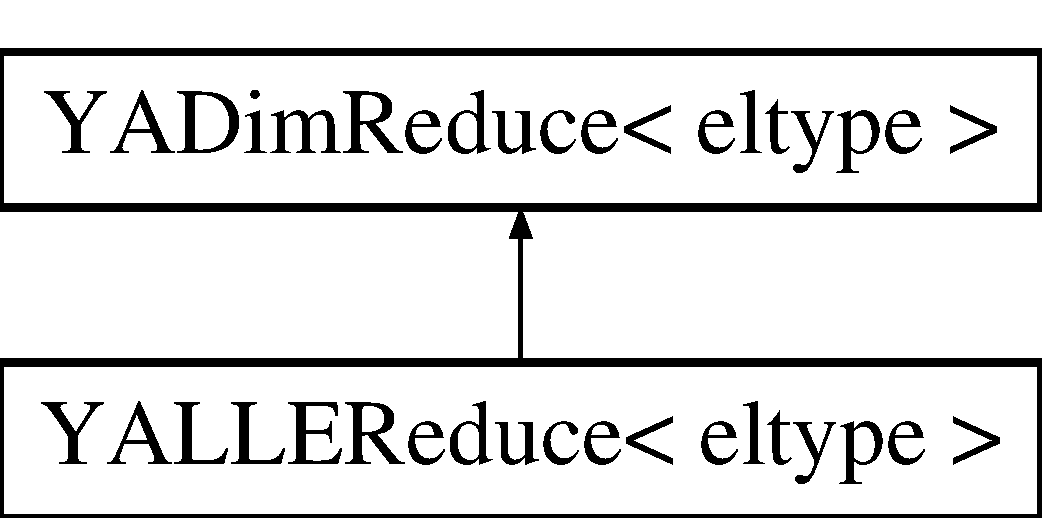
\includegraphics[height=2cm]{class_y_a_l_l_e_reduce}
\end{center}
\end{figure}
\subsection*{Public Member Functions}
\begin{CompactItemize}
\item 
\hypertarget{class_y_a_l_l_e_reduce_a2}{
const string \hyperlink{class_y_a_l_l_e_reduce_a2}{method\_\-name} () const }
\label{class_y_a_l_l_e_reduce_a2}

\begin{CompactList}\small\item\em Return the name of the dimensionality reduction method. \item\end{CompactList}\item 
\hypertarget{class_y_a_l_l_e_reduce_a3}{
const string \hyperlink{class_y_a_l_l_e_reduce_a3}{method\_\-id} () const }
\label{class_y_a_l_l_e_reduce_a3}

\begin{CompactList}\small\item\em Return the id of the dimensionality reduction method. \item\end{CompactList}\item 
\hypertarget{class_y_a_l_l_e_reduce_a4}{
const string \hyperlink{class_y_a_l_l_e_reduce_a4}{version} () const }
\label{class_y_a_l_l_e_reduce_a4}

\begin{CompactList}\small\item\em Return the version of the dimensionality reduction method. \item\end{CompactList}\item 
template$<$class mat\_\-type, class ya\_\-type2$>$ int \hyperlink{class_y_a_l_l_e_reduce_a5}{find\_\-map} (const YA\_\-Base\-T \&input, ya\_\-type2 \&output, ya\_\-sizet dim, Eigen\-Options \&eigopts)
\begin{CompactList}\small\item\em Find the reduction based on initial samples. \item\end{CompactList}\item 
\hypertarget{class_y_a_l_l_e_reduce_a6}{
template$<$class ya\_\-type1, class ya\_\-type2$>$ void \hyperlink{class_y_a_l_l_e_reduce_a6}{forward\_\-map} (const ya\_\-type1 \&input, ya\_\-type2 \&output) const }
\label{class_y_a_l_l_e_reduce_a6}

\begin{CompactList}\small\item\em Map in the forward direction to reduce the dimensionality of a matrix. \item\end{CompactList}\item 
\hypertarget{class_y_a_l_l_e_reduce_a7}{
template$<$class ya\_\-type1, class ya\_\-type2$>$ void \hyperlink{class_y_a_l_l_e_reduce_a7}{reverse\_\-map} (const ya\_\-type1 \&input, ya\_\-type2 \&output) const }
\label{class_y_a_l_l_e_reduce_a7}

\begin{CompactList}\small\item\em Map in the reverse direction to increase the dimensionality of a matrix. \item\end{CompactList}\item 
int \hyperlink{class_y_a_l_l_e_reduce_a8}{find} (const YA\_\-Mat\-T \&input, YA\_\-Mat\-T \&output, ya\_\-sizet dim, Eigen\-Options \&eigopts)
\begin{CompactList}\small\item\em Find the reduction based on initial samples. \item\end{CompactList}\item 
\hypertarget{class_y_a_l_l_e_reduce_a9}{
void \hyperlink{class_y_a_l_l_e_reduce_a9}{forward} (const YA\_\-Mat\-T \&input, YA\_\-Mat\-T \&output) const }
\label{class_y_a_l_l_e_reduce_a9}

\begin{CompactList}\small\item\em Map in the forward direction to reduce the dimensionality of a matrix. \item\end{CompactList}\item 
\hypertarget{class_y_a_l_l_e_reduce_a10}{
void \hyperlink{class_y_a_l_l_e_reduce_a10}{reverse} (const YA\_\-Mat\-T \&input, YA\_\-Mat\-T \&output) const }
\label{class_y_a_l_l_e_reduce_a10}

\begin{CompactList}\small\item\em Map in the reverse direction to increase the dimensionality of a matrix. \item\end{CompactList}\item 
\hypertarget{class_y_a_l_l_e_reduce_a11}{
void \hyperlink{class_y_a_l_l_e_reduce_a11}{save\_\-map} (ostream \&out) const }
\label{class_y_a_l_l_e_reduce_a11}

\begin{CompactList}\small\item\em Save a map to the given stream. \item\end{CompactList}\item 
\hypertarget{class_y_a_l_l_e_reduce_a12}{
int \hyperlink{class_y_a_l_l_e_reduce_a12}{load\_\-map} (istream \&in)}
\label{class_y_a_l_l_e_reduce_a12}

\begin{CompactList}\small\item\em Save a map from the given stream. \item\end{CompactList}\end{CompactItemize}


\subsection{Detailed Description}
\subsubsection*{template$<$class eltype$>$ class YALLEReduce$<$ eltype $>$}

Dimensionality reduction using Locally Linear Embedding. 

This implements the LLE dimensionality reduction algorithm described in:

S. Roweis and L. Saul, Science 290, 2323 (2000). 



\subsection{Member Function Documentation}
\hypertarget{class_y_a_l_l_e_reduce_a8}{
\index{YALLEReduce@{YALLEReduce}!find@{find}}
\index{find@{find}!YALLEReduce@{YALLEReduce}}
\subsubsection[find]{\setlength{\rightskip}{0pt plus 5cm}template$<$class eltype$>$ int \hyperlink{class_y_a_l_l_e_reduce}{YALLEReduce}$<$ eltype $>$::find (const YA\_\-Mat\-T \& {\em input}, YA\_\-Mat\-T \& {\em output}, ya\_\-sizet {\em dim}, Eigen\-Options \& {\em eigopts})\hspace{0.3cm}{\tt  \mbox{[}inline, virtual\mbox{]}}}}
\label{class_y_a_l_l_e_reduce_a8}


Find the reduction based on initial samples. 

\begin{Desc}
\item[Parameters:]
\begin{description}
\item[{\em input}]Matrix storing initial samples (columns are dimensions) \item[{\em output}]Matrix storing low-dimensioal coords of samples \item[{\em dim}]New dimensionality for output matrix $\ast$ \end{description}
\end{Desc}


Implements \hyperlink{class_y_a_dim_reduce_a8}{YADim\-Reduce$<$ eltype $>$}.\hypertarget{class_y_a_l_l_e_reduce_a5}{
\index{YALLEReduce@{YALLEReduce}!find_map@{find\_\-map}}
\index{find_map@{find\_\-map}!YALLEReduce@{YALLEReduce}}
\subsubsection[find\_\-map]{\setlength{\rightskip}{0pt plus 5cm}template$<$class eltype$>$ template$<$class mat\_\-type, class ya\_\-type2$>$ int \hyperlink{class_y_a_l_l_e_reduce}{YALLEReduce}$<$ eltype $>$::find\_\-map (const YA\_\-Base\-T \& {\em input}, ya\_\-type2 \& {\em output}, ya\_\-sizet {\em dim}, Eigen\-Options \& {\em eigopts})}}
\label{class_y_a_l_l_e_reduce_a5}


Find the reduction based on initial samples. 

\begin{Desc}
\item[Parameters:]
\begin{description}
\item[{\em input}]Symmetric matrix storing initial distances \item[{\em output}]Matrix storing low-dimensioal map of samples \item[{\em dim}]New dimensionality for output matrix $\ast$ \end{description}
\end{Desc}


The documentation for this class was generated from the following files:\begin{CompactItemize}
\item 
/tmp/drl/cpp/math/dimred/\hyperlink{ya__lle__reduce_8h}{ya\_\-lle\_\-reduce.h}\item 
/tmp/drl/cpp/math/dimred/ya\_\-lle\_\-reduce.cpp\end{CompactItemize}

\hypertarget{class_y_a_m_d_s_reduce}{
\section{YAMDSReduce$<$ eltype $>$ Class Template Reference}
\label{class_y_a_m_d_s_reduce}\index{YAMDSReduce@{YAMDSReduce}}
}
Dimensionality reduction using multidimensional scaling.  


{\tt \#include $<$ya\_\-mds\_\-reduce.h$>$}

Inheritance diagram for YAMDSReduce$<$ eltype $>$::\begin{figure}[H]
\begin{center}
\leavevmode
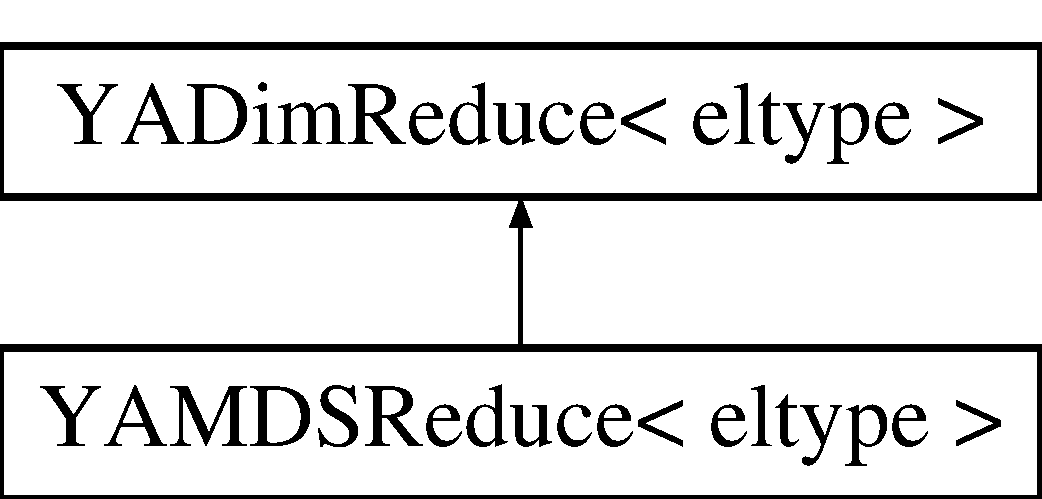
\includegraphics[height=2cm]{class_y_a_m_d_s_reduce}
\end{center}
\end{figure}
\subsection*{Public Member Functions}
\begin{CompactItemize}
\item 
\hypertarget{class_y_a_m_d_s_reduce_a2}{
const string \hyperlink{class_y_a_m_d_s_reduce_a2}{method\_\-name} () const }
\label{class_y_a_m_d_s_reduce_a2}

\begin{CompactList}\small\item\em Return the name of the dimensionality reduction method. \item\end{CompactList}\item 
\hypertarget{class_y_a_m_d_s_reduce_a3}{
const string \hyperlink{class_y_a_m_d_s_reduce_a3}{method\_\-id} () const }
\label{class_y_a_m_d_s_reduce_a3}

\begin{CompactList}\small\item\em Return the id of the dimensionality reduction method. \item\end{CompactList}\item 
\hypertarget{class_y_a_m_d_s_reduce_a4}{
const string \hyperlink{class_y_a_m_d_s_reduce_a4}{version} () const }
\label{class_y_a_m_d_s_reduce_a4}

\begin{CompactList}\small\item\em Return the version of the dimensionality reduction method. \item\end{CompactList}\item 
template$<$class ya\_\-type1, class ya\_\-type2$>$ int \hyperlink{class_y_a_m_d_s_reduce_a5}{find\_\-map} (const ya\_\-type1 \&input, ya\_\-type2 \&output, ya\_\-sizet dim, Eigen\-Options \&eigopts)
\begin{CompactList}\small\item\em Find the reduction based on initial samples. \item\end{CompactList}\item 
\hypertarget{class_y_a_m_d_s_reduce_a6}{
template$<$class ya\_\-type1, class ya\_\-type2$>$ void \hyperlink{class_y_a_m_d_s_reduce_a6}{forward\_\-map} (const ya\_\-type1 \&input, ya\_\-type2 \&output) const }
\label{class_y_a_m_d_s_reduce_a6}

\begin{CompactList}\small\item\em Map in the forward direction to reduce the dimensionality of a matrix. \item\end{CompactList}\item 
\hypertarget{class_y_a_m_d_s_reduce_a7}{
template$<$class ya\_\-type1, class ya\_\-type2$>$ void \hyperlink{class_y_a_m_d_s_reduce_a7}{reverse\_\-map} (const ya\_\-type1 \&input, ya\_\-type2 \&output) const }
\label{class_y_a_m_d_s_reduce_a7}

\begin{CompactList}\small\item\em Map in the reverse direction to increase the dimensionality of a matrix. \item\end{CompactList}\item 
int \hyperlink{class_y_a_m_d_s_reduce_a8}{find} (const YA\_\-Mat\-T \&input, YA\_\-Mat\-T \&output, ya\_\-sizet dim, Eigen\-Options \&eigopts)
\begin{CompactList}\small\item\em Find the reduction based on initial samples. \item\end{CompactList}\item 
\hypertarget{class_y_a_m_d_s_reduce_a9}{
void \hyperlink{class_y_a_m_d_s_reduce_a9}{forward} (const YA\_\-Mat\-T \&input, YA\_\-Mat\-T \&output) const }
\label{class_y_a_m_d_s_reduce_a9}

\begin{CompactList}\small\item\em Map in the forward direction to reduce the dimensionality of a matrix. \item\end{CompactList}\item 
\hypertarget{class_y_a_m_d_s_reduce_a10}{
void \hyperlink{class_y_a_m_d_s_reduce_a10}{reverse} (const YA\_\-Mat\-T \&input, YA\_\-Mat\-T \&output) const }
\label{class_y_a_m_d_s_reduce_a10}

\begin{CompactList}\small\item\em Map in the reverse direction to increase the dimensionality of a matrix. \item\end{CompactList}\item 
\hypertarget{class_y_a_m_d_s_reduce_a11}{
void \hyperlink{class_y_a_m_d_s_reduce_a11}{save\_\-map} (ostream \&out) const }
\label{class_y_a_m_d_s_reduce_a11}

\begin{CompactList}\small\item\em Save a map to the given stream. \item\end{CompactList}\item 
\hypertarget{class_y_a_m_d_s_reduce_a12}{
int \hyperlink{class_y_a_m_d_s_reduce_a12}{load\_\-map} (istream \&in)}
\label{class_y_a_m_d_s_reduce_a12}

\begin{CompactList}\small\item\em Load a map from the given stream. \item\end{CompactList}\end{CompactItemize}


\subsection{Detailed Description}
\subsubsection*{template$<$class eltype$>$ class YAMDSReduce$<$ eltype $>$}

Dimensionality reduction using multidimensional scaling. 



\subsection{Member Function Documentation}
\hypertarget{class_y_a_m_d_s_reduce_a8}{
\index{YAMDSReduce@{YAMDSReduce}!find@{find}}
\index{find@{find}!YAMDSReduce@{YAMDSReduce}}
\subsubsection[find]{\setlength{\rightskip}{0pt plus 5cm}template$<$class eltype$>$ int \hyperlink{class_y_a_m_d_s_reduce}{YAMDSReduce}$<$ eltype $>$::find (const YA\_\-Mat\-T \& {\em input}, YA\_\-Mat\-T \& {\em output}, ya\_\-sizet {\em dim}, Eigen\-Options \& {\em eigopts})\hspace{0.3cm}{\tt  \mbox{[}inline, virtual\mbox{]}}}}
\label{class_y_a_m_d_s_reduce_a8}


Find the reduction based on initial samples. 

\begin{Desc}
\item[Parameters:]
\begin{description}
\item[{\em input}]Matrix storing initial samples (columns are dimensions) \item[{\em output}]Matrix storing low-dimensioal coords of samples \item[{\em dim}]New dimensionality for output matrix $\ast$ \end{description}
\end{Desc}


Implements \hyperlink{class_y_a_dim_reduce_a8}{YADim\-Reduce$<$ eltype $>$}.\hypertarget{class_y_a_m_d_s_reduce_a5}{
\index{YAMDSReduce@{YAMDSReduce}!find_map@{find\_\-map}}
\index{find_map@{find\_\-map}!YAMDSReduce@{YAMDSReduce}}
\subsubsection[find\_\-map]{\setlength{\rightskip}{0pt plus 5cm}template$<$class eltype$>$ template$<$class ya\_\-type1, class ya\_\-type2$>$ YALANAMESPACE int \hyperlink{class_y_a_m_d_s_reduce}{YAMDSReduce}$<$ eltype $>$::find\_\-map (const ya\_\-type1 \& {\em input}, ya\_\-type2 \& {\em output}, ya\_\-sizet {\em dim}, Eigen\-Options \& {\em eigopts})}}
\label{class_y_a_m_d_s_reduce_a5}


Find the reduction based on initial samples. 

\begin{Desc}
\item[Parameters:]
\begin{description}
\item[{\em input}]Symmetric matrix storing initial distances \item[{\em output}]Matrix storing low-dimensioal coords of samples \item[{\em dim}]New dimensionality for output matrix $\ast$ \end{description}
\end{Desc}


The documentation for this class was generated from the following files:\begin{CompactItemize}
\item 
/tmp/drl/cpp/math/dimred/\hyperlink{ya__mds__reduce_8h}{ya\_\-mds\_\-reduce.h}\item 
/tmp/drl/cpp/math/dimred/ya\_\-mds\_\-reduce.cpp\end{CompactItemize}

\hypertarget{class_y_a_p_c_a_reduce}{
\section{YAPCAReduce$<$ eltype $>$ Class Template Reference}
\label{class_y_a_p_c_a_reduce}\index{YAPCAReduce@{YAPCAReduce}}
}
Dimensionality reduction using principal component analysis.  


{\tt \#include $<$ya\_\-pca\_\-reduce.h$>$}

Inheritance diagram for YAPCAReduce$<$ eltype $>$::\begin{figure}[H]
\begin{center}
\leavevmode
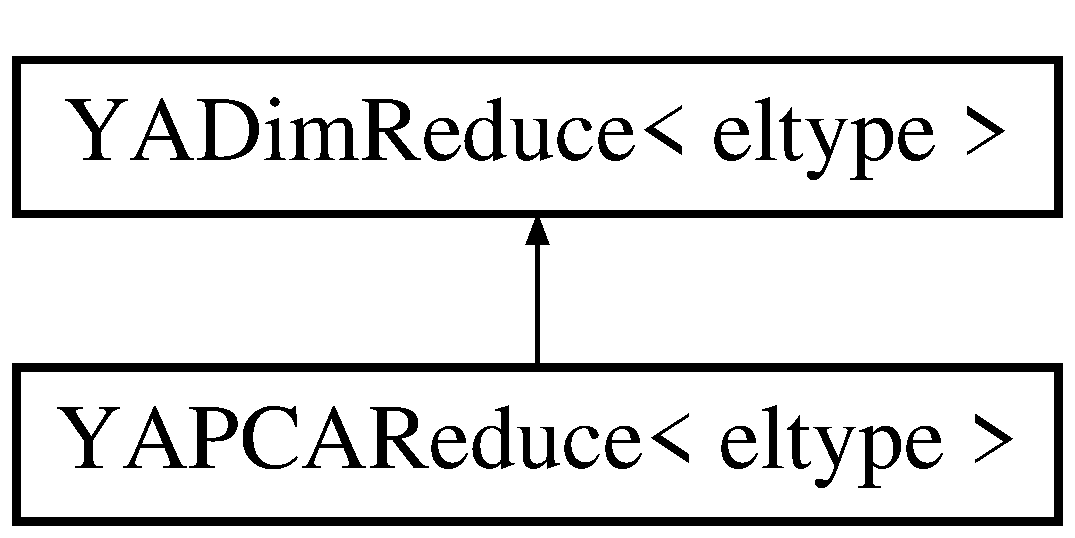
\includegraphics[height=2cm]{class_y_a_p_c_a_reduce}
\end{center}
\end{figure}
\subsection*{Public Member Functions}
\begin{CompactItemize}
\item 
\hypertarget{class_y_a_p_c_a_reduce_a2}{
const string \hyperlink{class_y_a_p_c_a_reduce_a2}{method\_\-name} () const }
\label{class_y_a_p_c_a_reduce_a2}

\begin{CompactList}\small\item\em Return the name of the dimensionality reduction method. \item\end{CompactList}\item 
\hypertarget{class_y_a_p_c_a_reduce_a3}{
const string \hyperlink{class_y_a_p_c_a_reduce_a3}{method\_\-id} () const }
\label{class_y_a_p_c_a_reduce_a3}

\begin{CompactList}\small\item\em Return the id of the dimensionality reduction method. \item\end{CompactList}\item 
\hypertarget{class_y_a_p_c_a_reduce_a4}{
const string \hyperlink{class_y_a_p_c_a_reduce_a4}{version} () const }
\label{class_y_a_p_c_a_reduce_a4}

\begin{CompactList}\small\item\em Return the version of the dimensionality reduction method. \item\end{CompactList}\item 
template$<$class ya\_\-type1, class ya\_\-type2$>$ int \hyperlink{class_y_a_p_c_a_reduce_a5}{find\_\-map} (const ya\_\-type1 \&input, ya\_\-type2 \&output, ya\_\-sizet dim, Eigen\-Options \&eigopts)
\begin{CompactList}\small\item\em Find the map for reduction based on initial samples. \item\end{CompactList}\item 
\hypertarget{class_y_a_p_c_a_reduce_a6}{
template$<$class ya\_\-type1, class ya\_\-type2$>$ void \hyperlink{class_y_a_p_c_a_reduce_a6}{forward\_\-map} (const ya\_\-type1 \&input, ya\_\-type2 \&output) const }
\label{class_y_a_p_c_a_reduce_a6}

\begin{CompactList}\small\item\em Map in the forward direction to reduce the dimensionality of a matrix. \item\end{CompactList}\item 
\hypertarget{class_y_a_p_c_a_reduce_a7}{
template$<$class ya\_\-type1, class ya\_\-type2$>$ void \hyperlink{class_y_a_p_c_a_reduce_a7}{reverse\_\-map} (const ya\_\-type1 \&input, ya\_\-type2 \&output) const }
\label{class_y_a_p_c_a_reduce_a7}

\begin{CompactList}\small\item\em Map in the reverse direction to increase the dimensionality of a matrix. \item\end{CompactList}\item 
int \hyperlink{class_y_a_p_c_a_reduce_a8}{find} (const YA\_\-Mat\-T \&input, YA\_\-Mat\-T \&output, ya\_\-sizet dim, Eigen\-Options \&eigopts)
\begin{CompactList}\small\item\em Find the map for reduction based on initial samples. \item\end{CompactList}\item 
\hypertarget{class_y_a_p_c_a_reduce_a9}{
void \hyperlink{class_y_a_p_c_a_reduce_a9}{forward} (const YA\_\-Mat\-T \&input, YA\_\-Mat\-T \&output) const }
\label{class_y_a_p_c_a_reduce_a9}

\begin{CompactList}\small\item\em Map in the forward direction to reduce the dimensionality of a matrix. \item\end{CompactList}\item 
\hypertarget{class_y_a_p_c_a_reduce_a10}{
void \hyperlink{class_y_a_p_c_a_reduce_a10}{reverse} (const YA\_\-Mat\-T \&input, YA\_\-Mat\-T \&output) const }
\label{class_y_a_p_c_a_reduce_a10}

\begin{CompactList}\small\item\em Map in the reverse direction to increase the dimensionality of a matrix. \item\end{CompactList}\item 
template$<$class ya\_\-type1, class ya\_\-type2, class ya\_\-type3, class ya\_\-type4$>$ void \hyperlink{class_y_a_p_c_a_reduce_a11}{reconstruct\_\-error} (const ya\_\-type1 \&input, const ya\_\-type2 \&output, const ya\_\-type3 \&dims, ya\_\-type4 \&rmsd)
\begin{CompactList}\small\item\em Get the reconstruction errors for the given low dimensionalities. \item\end{CompactList}\item 
\hypertarget{class_y_a_p_c_a_reduce_a12}{
void \hyperlink{class_y_a_p_c_a_reduce_a12}{save\_\-map} (ostream \&out) const }
\label{class_y_a_p_c_a_reduce_a12}

\begin{CompactList}\small\item\em Save a map to the given stream. \item\end{CompactList}\item 
\hypertarget{class_y_a_p_c_a_reduce_a13}{
int \hyperlink{class_y_a_p_c_a_reduce_a13}{load\_\-map} (istream \&in)}
\label{class_y_a_p_c_a_reduce_a13}

\begin{CompactList}\small\item\em Load a map from the given stream. \item\end{CompactList}\end{CompactItemize}


\subsection{Detailed Description}
\subsubsection*{template$<$class eltype$>$ class YAPCAReduce$<$ eltype $>$}

Dimensionality reduction using principal component analysis. 



\subsection{Member Function Documentation}
\hypertarget{class_y_a_p_c_a_reduce_a8}{
\index{YAPCAReduce@{YAPCAReduce}!find@{find}}
\index{find@{find}!YAPCAReduce@{YAPCAReduce}}
\subsubsection[find]{\setlength{\rightskip}{0pt plus 5cm}template$<$class eltype$>$ int \hyperlink{class_y_a_p_c_a_reduce}{YAPCAReduce}$<$ eltype $>$::find (const YA\_\-Mat\-T \& {\em input}, YA\_\-Mat\-T \& {\em output}, ya\_\-sizet {\em dim}, Eigen\-Options \& {\em eigopts})\hspace{0.3cm}{\tt  \mbox{[}inline, virtual\mbox{]}}}}
\label{class_y_a_p_c_a_reduce_a8}


Find the map for reduction based on initial samples. 

\begin{Desc}
\item[Parameters:]
\begin{description}
\item[{\em input}]Matrix storing initial samples (columns are dimensions) \item[{\em output}]Matrix storing low-dimensioal coords of samples \item[{\em dim}]New dimensionality for output matrix $\ast$ \end{description}
\end{Desc}


Implements \hyperlink{class_y_a_dim_reduce_a8}{YADim\-Reduce$<$ eltype $>$}.\hypertarget{class_y_a_p_c_a_reduce_a5}{
\index{YAPCAReduce@{YAPCAReduce}!find_map@{find\_\-map}}
\index{find_map@{find\_\-map}!YAPCAReduce@{YAPCAReduce}}
\subsubsection[find\_\-map]{\setlength{\rightskip}{0pt plus 5cm}template$<$class eltype$>$ template$<$class ya\_\-type1, class ya\_\-type2$>$ YALANAMESPACE int \hyperlink{class_y_a_p_c_a_reduce}{YAPCAReduce}$<$ eltype $>$::find\_\-map (const ya\_\-type1 \& {\em input}, ya\_\-type2 \& {\em output}, ya\_\-sizet {\em dim}, Eigen\-Options \& {\em eigopts})}}
\label{class_y_a_p_c_a_reduce_a5}


Find the map for reduction based on initial samples. 

\begin{Desc}
\item[Parameters:]
\begin{description}
\item[{\em input}]Matrix storing initial samples (columns are dimensions) \item[{\em output}]Matrix storing low-dimensioal coords of samples \item[{\em dim}]New dimensionality for output matrix $\ast$ \end{description}
\end{Desc}
\hypertarget{class_y_a_p_c_a_reduce_a11}{
\index{YAPCAReduce@{YAPCAReduce}!reconstruct_error@{reconstruct\_\-error}}
\index{reconstruct_error@{reconstruct\_\-error}!YAPCAReduce@{YAPCAReduce}}
\subsubsection[reconstruct\_\-error]{\setlength{\rightskip}{0pt plus 5cm}template$<$class eltype$>$ template$<$class ya\_\-type1, class ya\_\-type2, class ya\_\-type3, class ya\_\-type4$>$ void \hyperlink{class_y_a_p_c_a_reduce}{YAPCAReduce}$<$ eltype $>$::reconstruct\_\-error (const ya\_\-type1 \& {\em input}, const ya\_\-type2 \& {\em output}, const ya\_\-type3 \& {\em dims}, ya\_\-type4 \& {\em rmsd})}}
\label{class_y_a_p_c_a_reduce_a11}


Get the reconstruction errors for the given low dimensionalities. 

\begin{Desc}
\item[Parameters:]
\begin{description}
\item[{\em input}]High dimensional coordinates \item[{\em output}]Low dimensional coordinates \item[{\em dims}]SORTED Dimensionalities to calculate the reconstruction errors \item[{\em rmsd}]Root mean squared deviations for reconstruction errors $\ast$ \end{description}
\end{Desc}


The documentation for this class was generated from the following files:\begin{CompactItemize}
\item 
/tmp/drl/cpp/math/dimred/\hyperlink{ya__pca__reduce_8h}{ya\_\-pca\_\-reduce.h}\item 
/tmp/drl/cpp/math/dimred/ya\_\-pca\_\-reduce.cpp\end{CompactItemize}

\chapter{Dr.L. File Documentation}
\hypertarget{drl__doxygen_8h}{
\section{/tmp/drl/cpp/math/dimred/drl\_\-doxygen.h File Reference}
\label{drl__doxygen_8h}\index{/tmp/drl/cpp/math/dimred/drl_doxygen.h@{/tmp/drl/cpp/math/dimred/drl\_\-doxygen.h}}
}


\subsection{Detailed Description}

\hypertarget{ya__dim__redfun_8h}{
\section{/tmp/drl/cpp/math/dimred/ya\_\-dim\_\-redfun.h File Reference}
\label{ya__dim__redfun_8h}\index{/tmp/drl/cpp/math/dimred/ya_dim_redfun.h@{/tmp/drl/cpp/math/dimred/ya\_\-dim\_\-redfun.h}}
}
\subsection*{Functions}
\begin{CompactItemize}
\item 
template$<$class eltype, class mat\_\-type, class ya\_\-type2$>$ YALANAMESPACE void \hyperlink{ya__dim__redfun_8h_a0}{point\_\-pca} (const YA\_\-Base\-T \&input, const ya\_\-sizet k, Eigen\-Options \&eigopts, ya\_\-type2 \&output, const int verbose)
\begin{CompactList}\small\item\em Return a n x d matrix of residual variances for n points from PCA. \item\end{CompactList}\item 
template$<$class eltype, class mat\_\-type, class ya\_\-type2, class ya\_\-type3$>$ void \hyperlink{ya__dim__redfun_8h_a1}{point\_\-pca} (const YA\_\-Base\-T \&input, const ya\_\-sizet k, const ya\_\-type2 \&dims, Eigen\-Options \&eigopts, ya\_\-type3 \&output, const int verbose)
\begin{CompactList}\small\item\em Return a n x d matrix of residual variances for n points from PCA. \item\end{CompactList}\item 
template$<$class eltype, class mat\_\-type, class ya\_\-type2$>$ void \hyperlink{ya__dim__redfun_8h_a2}{point\_\-pca\_\-ep} (const YA\_\-Base\-T \&input, const eltype epsilon, Eigen\-Options \&eigopts, ya\_\-type2 \&output, const int verbose)
\begin{CompactList}\small\item\em Same as point\_\-pca except epsilon nearest neighbors is used. \item\end{CompactList}\item 
template$<$class eltype, class mat\_\-type, class ya\_\-type2, class ya\_\-type3$>$ void \hyperlink{ya__dim__redfun_8h_a3}{point\_\-pca\_\-ep} (const YA\_\-Base\-T \&input, const eltype epsilon, const ya\_\-type2 \&dims, Eigen\-Options \&eigopts, ya\_\-type3 \&output, const int verbose)
\begin{CompactList}\small\item\em Same as point\_\-pca except epsilon nearest neighbors is used. \item\end{CompactList}\item 
template$<$class eltype, class mat\_\-type$>$ void \hyperlink{ya__dim__redfun_8h_a4}{point\_\-pca} (const YA\_\-Base\-T \&input, const ya\_\-sizet k, Eigen\-Options \&eigopts, YA\_\-Row\-D \&vmean, YA\_\-Row\-D \&vmin, YA\_\-Row\-D \&vmax, YA\_\-Row\-D \&vstd, const int verbose)
\begin{CompactList}\small\item\em Return statistics of residual variances for n points from PCA. \item\end{CompactList}\item 
template$<$class eltype, class mat\_\-type, class ya\_\-type2$>$ void \hyperlink{ya__dim__redfun_8h_a5}{point\_\-pca} (const YA\_\-Base\-T \&input, const ya\_\-sizet k, const ya\_\-type2 \&dims, Eigen\-Options \&eigopts, YA\_\-Row\-D \&vmean, YA\_\-Row\-D \&vmin, YA\_\-Row\-D \&vmax, YA\_\-Row\-D \&vstd, const int verbose)
\begin{CompactList}\small\item\em Return statistics of residual variances for n points from PCA. \item\end{CompactList}\item 
template$<$class eltype, class mat\_\-type$>$ void \hyperlink{ya__dim__redfun_8h_a6}{point\_\-pca\_\-ep} (const YA\_\-Base\-T \&input, const eltype epsilon, Eigen\-Options \&eigopts, YA\_\-Row\-D \&vmean, YA\_\-Row\-D \&vmin, YA\_\-Row\-D \&vmax, YA\_\-Row\-D \&vstd, const int verbose)
\begin{CompactList}\small\item\em Same as point\_\-pca except epsilon nearest neighbors is used. \item\end{CompactList}\item 
template$<$class eltype, class mat\_\-type, class ya\_\-type2$>$ void \hyperlink{ya__dim__redfun_8h_a7}{point\_\-pca\_\-ep} (const YA\_\-Base\-T \&input, const eltype epsilon, const ya\_\-type2 \&dims, Eigen\-Options \&eigopts, YA\_\-Row\-D \&vmean, YA\_\-Row\-D \&vmin, YA\_\-Row\-D \&vmax, YA\_\-Row\-D \&vstd, const int verbose)
\begin{CompactList}\small\item\em Same as point\_\-pca except epsilon nearest neighbors is used. \item\end{CompactList}\end{CompactItemize}


\subsection{Detailed Description}


\subsection{Function Documentation}
\hypertarget{ya__dim__redfun_8h_a5}{
\index{ya_dim_redfun.h@{ya\_\-dim\_\-redfun.h}!point_pca@{point\_\-pca}}
\index{point_pca@{point\_\-pca}!ya_dim_redfun.h@{ya\_\-dim\_\-redfun.h}}
\subsubsection[point\_\-pca]{\setlength{\rightskip}{0pt plus 5cm}template$<$class eltype, class mat\_\-type, class ya\_\-type2$>$ void point\_\-pca (const YA\_\-Base\-T \& {\em input}, const ya\_\-sizet {\em k}, const ya\_\-type2 \& {\em dims}, Eigen\-Options \& {\em eigopts}, YA\_\-Row\-D \& {\em vmean}, YA\_\-Row\-D \& {\em vmin}, YA\_\-Row\-D \& {\em vmax}, YA\_\-Row\-D \& {\em vstd}, const int {\em verbose})}}
\label{ya__dim__redfun_8h_a5}


Return statistics of residual variances for n points from PCA. 

\begin{Desc}
\item[Parameters:]
\begin{description}
\item[{\em input}]n x d matrix of samples \item[{\em k}]Local PCA is performed on each point and its k nearest neighbors \item[{\em dims}]length D vector containing dimensions for statistics calculation \item[{\em vmean}]length D vector containing mean residual variance for each dim \item[{\em vmin}]length D vector containing min residual variance for each dim \item[{\em vmax}]length D vector containing max residual variance for each dim \item[{\em vstd}]length D vector containing std devation of residual variance \item[{\em verbose}]0 no output, 1 progress meter/timing, 2 also nbor stats $\ast$ \end{description}
\end{Desc}
\hypertarget{ya__dim__redfun_8h_a4}{
\index{ya_dim_redfun.h@{ya\_\-dim\_\-redfun.h}!point_pca@{point\_\-pca}}
\index{point_pca@{point\_\-pca}!ya_dim_redfun.h@{ya\_\-dim\_\-redfun.h}}
\subsubsection[point\_\-pca]{\setlength{\rightskip}{0pt plus 5cm}template$<$class eltype, class mat\_\-type$>$ void point\_\-pca (const YA\_\-Base\-T \& {\em input}, const ya\_\-sizet {\em k}, Eigen\-Options \& {\em eigopts}, YA\_\-Row\-D \& {\em vmean}, YA\_\-Row\-D \& {\em vmin}, YA\_\-Row\-D \& {\em vmax}, YA\_\-Row\-D \& {\em vstd}, const int {\em verbose})}}
\label{ya__dim__redfun_8h_a4}


Return statistics of residual variances for n points from PCA. 

\begin{Desc}
\item[Parameters:]
\begin{description}
\item[{\em input}]n x d matrix of samples \item[{\em k}]Local PCA is performed on each point and its k nearest neighbors \item[{\em vmean}]length d vector containing mean residual variance for each dim \item[{\em vmin}]length d vector containing min residual variance for each dim \item[{\em vmax}]length d vector containing max residual variance for each dim \item[{\em vstd}]length d vector containing std devation of residual variance \item[{\em verbose}]0 no output, 1 progress meter/timing, 2 also nbor stats $\ast$ \end{description}
\end{Desc}
\hypertarget{ya__dim__redfun_8h_a1}{
\index{ya_dim_redfun.h@{ya\_\-dim\_\-redfun.h}!point_pca@{point\_\-pca}}
\index{point_pca@{point\_\-pca}!ya_dim_redfun.h@{ya\_\-dim\_\-redfun.h}}
\subsubsection[point\_\-pca]{\setlength{\rightskip}{0pt plus 5cm}template$<$class eltype, class mat\_\-type, class ya\_\-type2, class ya\_\-type3$>$ void point\_\-pca (const YA\_\-Base\-T \& {\em input}, const ya\_\-sizet {\em k}, const ya\_\-type2 \& {\em dims}, Eigen\-Options \& {\em eigopts}, ya\_\-type3 \& {\em output}, const int {\em verbose})}}
\label{ya__dim__redfun_8h_a1}


Return a n x d matrix of residual variances for n points from PCA. 

\begin{Desc}
\item[Parameters:]
\begin{description}
\item[{\em dims}]length D vector of dimensionalities to include in calculation \item[{\em input}]n x D matrix of samples \item[{\em k}]Local PCA is performed on each point and its k nearest neighbors \item[{\em output}]n x D matrix of residual variances \item[{\em verbose}]0 no output, 1 progress meter/timing, 2 also nbor stats $\ast$ \end{description}
\end{Desc}
\hypertarget{ya__dim__redfun_8h_a0}{
\index{ya_dim_redfun.h@{ya\_\-dim\_\-redfun.h}!point_pca@{point\_\-pca}}
\index{point_pca@{point\_\-pca}!ya_dim_redfun.h@{ya\_\-dim\_\-redfun.h}}
\subsubsection[point\_\-pca]{\setlength{\rightskip}{0pt plus 5cm}template$<$class eltype, class mat\_\-type, class ya\_\-type2$>$ YALANAMESPACE void point\_\-pca (const YA\_\-Base\-T \& {\em input}, const ya\_\-sizet {\em k}, Eigen\-Options \& {\em eigopts}, ya\_\-type2 \& {\em output}, const int {\em verbose})}}
\label{ya__dim__redfun_8h_a0}


Return a n x d matrix of residual variances for n points from PCA. 

\begin{Desc}
\item[Parameters:]
\begin{description}
\item[{\em input}]n x d matrix of samples \item[{\em k}]Local PCA is performed on each point and its k nearest neighbors \item[{\em output}]n x d matrix of residual variances \item[{\em verbose}]0 no output, 1 progress meter/timing, 2 also nbor stats $\ast$ \end{description}
\end{Desc}
\hypertarget{ya__dim__redfun_8h_a7}{
\index{ya_dim_redfun.h@{ya\_\-dim\_\-redfun.h}!point_pca_ep@{point\_\-pca\_\-ep}}
\index{point_pca_ep@{point\_\-pca\_\-ep}!ya_dim_redfun.h@{ya\_\-dim\_\-redfun.h}}
\subsubsection[point\_\-pca\_\-ep]{\setlength{\rightskip}{0pt plus 5cm}template$<$class eltype, class mat\_\-type, class ya\_\-type2$>$ void point\_\-pca\_\-ep (const YA\_\-Base\-T \& {\em input}, const eltype {\em epsilon}, const ya\_\-type2 \& {\em dims}, Eigen\-Options \& {\em eigopts}, YA\_\-Row\-D \& {\em vmean}, YA\_\-Row\-D \& {\em vmin}, YA\_\-Row\-D \& {\em vmax}, YA\_\-Row\-D \& {\em vstd}, const int {\em verbose})}}
\label{ya__dim__redfun_8h_a7}


Same as point\_\-pca except epsilon nearest neighbors is used. 

\begin{Desc}
\item[See also:]\hyperlink{ya__dim__redfun_8h_a5}{point\_\-pca} $\ast$ \end{Desc}
\hypertarget{ya__dim__redfun_8h_a6}{
\index{ya_dim_redfun.h@{ya\_\-dim\_\-redfun.h}!point_pca_ep@{point\_\-pca\_\-ep}}
\index{point_pca_ep@{point\_\-pca\_\-ep}!ya_dim_redfun.h@{ya\_\-dim\_\-redfun.h}}
\subsubsection[point\_\-pca\_\-ep]{\setlength{\rightskip}{0pt plus 5cm}template$<$class eltype, class mat\_\-type$>$ void point\_\-pca\_\-ep (const YA\_\-Base\-T \& {\em input}, const eltype {\em epsilon}, Eigen\-Options \& {\em eigopts}, YA\_\-Row\-D \& {\em vmean}, YA\_\-Row\-D \& {\em vmin}, YA\_\-Row\-D \& {\em vmax}, YA\_\-Row\-D \& {\em vstd}, const int {\em verbose})}}
\label{ya__dim__redfun_8h_a6}


Same as point\_\-pca except epsilon nearest neighbors is used. 

\begin{Desc}
\item[See also:]\hyperlink{ya__dim__redfun_8h_a5}{point\_\-pca} $\ast$ \end{Desc}
\hypertarget{ya__dim__redfun_8h_a3}{
\index{ya_dim_redfun.h@{ya\_\-dim\_\-redfun.h}!point_pca_ep@{point\_\-pca\_\-ep}}
\index{point_pca_ep@{point\_\-pca\_\-ep}!ya_dim_redfun.h@{ya\_\-dim\_\-redfun.h}}
\subsubsection[point\_\-pca\_\-ep]{\setlength{\rightskip}{0pt plus 5cm}template$<$class eltype, class mat\_\-type, class ya\_\-type2, class ya\_\-type3$>$ void point\_\-pca\_\-ep (const YA\_\-Base\-T \& {\em input}, const eltype {\em epsilon}, const ya\_\-type2 \& {\em dims}, Eigen\-Options \& {\em eigopts}, ya\_\-type3 \& {\em output}, const int {\em verbose})}}
\label{ya__dim__redfun_8h_a3}


Same as point\_\-pca except epsilon nearest neighbors is used. 

\begin{Desc}
\item[See also:]\hyperlink{ya__dim__redfun_8h_a5}{point\_\-pca} $\ast$ \end{Desc}
\hypertarget{ya__dim__redfun_8h_a2}{
\index{ya_dim_redfun.h@{ya\_\-dim\_\-redfun.h}!point_pca_ep@{point\_\-pca\_\-ep}}
\index{point_pca_ep@{point\_\-pca\_\-ep}!ya_dim_redfun.h@{ya\_\-dim\_\-redfun.h}}
\subsubsection[point\_\-pca\_\-ep]{\setlength{\rightskip}{0pt plus 5cm}template$<$class eltype, class mat\_\-type, class ya\_\-type2$>$ void point\_\-pca\_\-ep (const YA\_\-Base\-T \& {\em input}, const eltype {\em epsilon}, Eigen\-Options \& {\em eigopts}, ya\_\-type2 \& {\em output}, const int {\em verbose})}}
\label{ya__dim__redfun_8h_a2}


Same as point\_\-pca except epsilon nearest neighbors is used. 

\begin{Desc}
\item[See also:]\hyperlink{ya__dim__redfun_8h_a5}{point\_\-pca} $\ast$ \end{Desc}

\hypertarget{ya__dim__reduce_8h}{
\section{/tmp/drl/cpp/math/dimred/ya\_\-dim\_\-reduce.h File Reference}
\label{ya__dim__reduce_8h}\index{/tmp/drl/cpp/math/dimred/ya_dim_reduce.h@{/tmp/drl/cpp/math/dimred/ya\_\-dim\_\-reduce.h}}
}
\subsection*{Classes}
\begin{CompactItemize}
\item 
class \hyperlink{class_y_a_dim_reduce}{YADim\-Reduce$<$ eltype $>$}
\begin{CompactList}\small\item\em General Base Class for Dimensionality Reduction. \item\end{CompactList}\end{CompactItemize}


\subsection{Detailed Description}

\hypertarget{ya__iso__reduce_8h}{
\section{/tmp/drl/cpp/math/dimred/ya\_\-iso\_\-reduce.h File Reference}
\label{ya__iso__reduce_8h}\index{/tmp/drl/cpp/math/dimred/ya_iso_reduce.h@{/tmp/drl/cpp/math/dimred/ya\_\-iso\_\-reduce.h}}
}
\subsection*{Classes}
\begin{CompactItemize}
\item 
class \hyperlink{class_y_a_iso_reduce}{YAIso\-Reduce$<$ eltype $>$}
\begin{CompactList}\small\item\em Dimensionality reduction using Iso\-Map. \item\end{CompactList}\end{CompactItemize}


\subsection{Detailed Description}

\hypertarget{ya__lle__reduce_8h}{
\section{/tmp/drl/cpp/math/dimred/ya\_\-lle\_\-reduce.h File Reference}
\label{ya__lle__reduce_8h}\index{/tmp/drl/cpp/math/dimred/ya_lle_reduce.h@{/tmp/drl/cpp/math/dimred/ya\_\-lle\_\-reduce.h}}
}
\subsection*{Classes}
\begin{CompactItemize}
\item 
class \hyperlink{class_y_a_l_l_e_reduce}{YALLEReduce$<$ eltype $>$}
\begin{CompactList}\small\item\em Dimensionality reduction using Locally Linear Embedding. \item\end{CompactList}\end{CompactItemize}


\subsection{Detailed Description}

\hypertarget{ya__mds__reduce_8h}{
\section{/tmp/drl/cpp/math/dimred/ya\_\-mds\_\-reduce.h File Reference}
\label{ya__mds__reduce_8h}\index{/tmp/drl/cpp/math/dimred/ya_mds_reduce.h@{/tmp/drl/cpp/math/dimred/ya\_\-mds\_\-reduce.h}}
}
\subsection*{Classes}
\begin{CompactItemize}
\item 
class \hyperlink{class_y_a_m_d_s_reduce}{YAMDSReduce$<$ eltype $>$}
\begin{CompactList}\small\item\em Dimensionality reduction using multidimensional scaling. \item\end{CompactList}\end{CompactItemize}


\subsection{Detailed Description}

\hypertarget{ya__pca__reduce_8h}{
\section{/tmp/drl/cpp/math/dimred/ya\_\-pca\_\-reduce.h File Reference}
\label{ya__pca__reduce_8h}\index{/tmp/drl/cpp/math/dimred/ya_pca_reduce.h@{/tmp/drl/cpp/math/dimred/ya\_\-pca\_\-reduce.h}}
}
\subsection*{Classes}
\begin{CompactItemize}
\item 
class \hyperlink{class_y_a_p_c_a_reduce}{YAPCAReduce$<$ eltype $>$}
\begin{CompactList}\small\item\em Dimensionality reduction using principal component analysis. \item\end{CompactList}\end{CompactItemize}


\subsection{Detailed Description}

\printindex
\end{document}
